%!TEX TS-program = xelatex
\documentclass[10pt,oneside]{article}

\usepackage[english]{babel}

\usepackage{amsmath,amssymb,amsfonts}
\usepackage[utf8]{inputenc}
\usepackage[T1]{fontenc}
\usepackage{stix}
\usepackage[scaled]{helvet}
\usepackage[scaled]{inconsolata}

\usepackage{lastpage}

\usepackage{setspace}

\usepackage{ccicons}

\usepackage[hang,flushmargin]{footmisc}

\usepackage{geometry}

\setlength{\parindent}{0pt}
\setlength{\parskip}{6pt plus 2pt minus 1pt}

\usepackage{fancyhdr}
\renewcommand{\headrulewidth}{0pt}\providecommand{\tightlist}{%
  \setlength{\itemsep}{0pt}\setlength{\parskip}{0pt}}

\makeatletter
\newcounter{tableno}
\newenvironment{tablenos:no-prefix-table-caption}{
  \caption@ifcompatibility{}{
    \let\oldthetable\thetable
    \let\oldtheHtable\theHtable
    \renewcommand{\thetable}{tableno:\thetableno}
    \renewcommand{\theHtable}{tableno:\thetableno}
    \stepcounter{tableno}
    \captionsetup{labelformat=empty}
  }
}{
  \caption@ifcompatibility{}{
    \captionsetup{labelformat=default}
    \let\thetable\oldthetable
    \let\theHtable\oldtheHtable
    \addtocounter{table}{-1}
  }
}
\makeatother

\usepackage{array}
\newcommand{\PreserveBackslash}[1]{\let\temp=\\#1\let\\=\temp}
\let\PBS=\PreserveBackslash

\usepackage[breaklinks=true]{hyperref}
\hypersetup{colorlinks,%
citecolor=blue,%
filecolor=blue,%
linkcolor=blue,%
urlcolor=blue}
\usepackage{url}

\usepackage{caption}
\setcounter{secnumdepth}{0}
\usepackage{cleveref}

\usepackage{graphicx}
\makeatletter
\def\maxwidth{\ifdim\Gin@nat@width>\linewidth\linewidth
\else\Gin@nat@width\fi}
\makeatother
\let\Oldincludegraphics\includegraphics
\renewcommand{\includegraphics}[1]{\Oldincludegraphics[width=\maxwidth]{#1}}

\usepackage{longtable}
\usepackage{booktabs}

\usepackage{color}
\usepackage{fancyvrb}
\newcommand{\VerbBar}{|}
\newcommand{\VERB}{\Verb[commandchars=\\\{\}]}
\DefineVerbatimEnvironment{Highlighting}{Verbatim}{commandchars=\\\{\}}
% Add ',fontsize=\small' for more characters per line
\usepackage{framed}
\definecolor{shadecolor}{RGB}{248,248,248}
\newenvironment{Shaded}{\begin{snugshade}}{\end{snugshade}}
\newcommand{\KeywordTok}[1]{\textcolor[rgb]{0.13,0.29,0.53}{\textbf{#1}}}
\newcommand{\DataTypeTok}[1]{\textcolor[rgb]{0.13,0.29,0.53}{#1}}
\newcommand{\DecValTok}[1]{\textcolor[rgb]{0.00,0.00,0.81}{#1}}
\newcommand{\BaseNTok}[1]{\textcolor[rgb]{0.00,0.00,0.81}{#1}}
\newcommand{\FloatTok}[1]{\textcolor[rgb]{0.00,0.00,0.81}{#1}}
\newcommand{\ConstantTok}[1]{\textcolor[rgb]{0.00,0.00,0.00}{#1}}
\newcommand{\CharTok}[1]{\textcolor[rgb]{0.31,0.60,0.02}{#1}}
\newcommand{\SpecialCharTok}[1]{\textcolor[rgb]{0.00,0.00,0.00}{#1}}
\newcommand{\StringTok}[1]{\textcolor[rgb]{0.31,0.60,0.02}{#1}}
\newcommand{\VerbatimStringTok}[1]{\textcolor[rgb]{0.31,0.60,0.02}{#1}}
\newcommand{\SpecialStringTok}[1]{\textcolor[rgb]{0.31,0.60,0.02}{#1}}
\newcommand{\ImportTok}[1]{#1}
\newcommand{\CommentTok}[1]{\textcolor[rgb]{0.56,0.35,0.01}{\textit{#1}}}
\newcommand{\DocumentationTok}[1]{\textcolor[rgb]{0.56,0.35,0.01}{\textbf{\textit{#1}}}}
\newcommand{\AnnotationTok}[1]{\textcolor[rgb]{0.56,0.35,0.01}{\textbf{\textit{#1}}}}
\newcommand{\CommentVarTok}[1]{\textcolor[rgb]{0.56,0.35,0.01}{\textbf{\textit{#1}}}}
\newcommand{\OtherTok}[1]{\textcolor[rgb]{0.56,0.35,0.01}{#1}}
\newcommand{\FunctionTok}[1]{\textcolor[rgb]{0.00,0.00,0.00}{#1}}
\newcommand{\VariableTok}[1]{\textcolor[rgb]{0.00,0.00,0.00}{#1}}
\newcommand{\ControlFlowTok}[1]{\textcolor[rgb]{0.13,0.29,0.53}{\textbf{#1}}}
\newcommand{\OperatorTok}[1]{\textcolor[rgb]{0.81,0.36,0.00}{\textbf{#1}}}
\newcommand{\BuiltInTok}[1]{#1}
\newcommand{\ExtensionTok}[1]{#1}
\newcommand{\PreprocessorTok}[1]{\textcolor[rgb]{0.56,0.35,0.01}{\textit{#1}}}
\newcommand{\AttributeTok}[1]{\textcolor[rgb]{0.77,0.63,0.00}{#1}}
\newcommand{\RegionMarkerTok}[1]{#1}
\newcommand{\InformationTok}[1]{\textcolor[rgb]{0.56,0.35,0.01}{\textbf{\textit{#1}}}}
\newcommand{\WarningTok}[1]{\textcolor[rgb]{0.56,0.35,0.01}{\textbf{\textit{#1}}}}
\newcommand{\AlertTok}[1]{\textcolor[rgb]{0.94,0.16,0.16}{#1}}
\newcommand{\ErrorTok}[1]{\textcolor[rgb]{0.64,0.00,0.00}{\textbf{#1}}}
\newcommand{\NormalTok}[1]{#1}

\newlength{\cslhangindent}
\setlength{\cslhangindent}{1.5em}
\newlength{\csllabelwidth}
\setlength{\csllabelwidth}{3em}
\newenvironment{CSLReferences}[3] % #1 hanging-ident, #2 entry spacing
 {% don't indent paragraphs
  \setlength{\parindent}{0pt}
  % turn on hanging indent if param 1 is 1
  \ifodd #1 \everypar{\setlength{\hangindent}{\cslhangindent}}\ignorespaces\fi
  % set entry spacing
  \ifnum #2 > 0
  \setlength{\parskip}{#2\baselineskip}
  \fi
 }%
 {}
\usepackage{calc} % for \widthof, \maxof
\newcommand{\CSLBlock}[1]{#1\hfill\break}
\newcommand{\CSLLeftMargin}[1]{\parbox[t]{\maxof{\widthof{#1}}{\csllabelwidth}}{#1}}
\newcommand{\CSLRightInline}[1]{\parbox[t]{\linewidth}{#1}}
\newcommand{\CSLIndent}[1]{\hspace{\cslhangindent}#1}\usepackage[table,dvipsnames]{xcolor}

\geometry{includemp,
            letterpaper,
            top=1.2in,
            bottom=2.510cm,
            inner=0.5in,
            outer=0.4in,
            marginparwidth=1.95in,
            marginparsep=0.4in}

\usepackage[singlelinecheck=off]{caption}
\captionsetup{
  font={small},
  labelfont={bf},
  format=plain,
  labelsep=quad
}
\usepackage{floatrow}
\floatsetup[figure]{margins=hangright,
              facing=no,
              capposition=beside,
              capbesideposition={center,outside},
              floatwidth=\textwidth}
\floatsetup[table]{margins=hangoutside,
             facing=yes,
             capposition=beside,
             capbesideposition={center,outside},
             floatwidth=\textwidth}

\pagestyle{plain}

\setcounter{secnumdepth}{5}

\usepackage{titlesec}

\titleformat{\section}[block]
{\normalfont\large\sffamily}
{\thesection}{.5em}{\titlerule\\[.8ex]\bfseries}

\titleformat{\subsection}[runin]
{\normalfont\fontseries{b}\selectfont\filright\sffamily}
{\thesubsection.}{.5em}{}

\titleformat{\subsubsection}[runin]
{\normalfont\itshape\rmfamily\bfseries}{\thesubsubsection}{1em}{}

\fancypagestyle{firstpage}
{
   \fancyhf{}
   \renewcommand{\headrulewidth}{0pt}
   \fancyfoot[R]{\footnotesize\ccby}
   \fancyfoot[L]{\footnotesize\sffamily\today}
}

\fancypagestyle{normal}
{
  \fancyhf{}
  \fancyfoot[R]{\footnotesize\sffamily\thepage\ of \pageref*{LastPage}}
}

\usepackage{tikz}
\begin{document}
\tikz [remember picture, overlay] %
\node [shift={(-0.6in,1.1cm)},scale=0.2,opacity=0.4] at (current page.south east)[anchor=south east]{
\includegraphics{logo}};%
\pagestyle{normal}
\thispagestyle{firstpage}

\newcommand{\colorRule}[3][black]{\textcolor[HTML]{#1}{\rule{#2}{#3}}}

\noindent {\LARGE \textbf{\textsf{Mismatch between IUCN range maps and
species interactions data illustrated using the Serengeti food web}}}

\medskip
\begin{flushleft}
{\small
%
\href{https://orcid.org/0000-0003-2791-8383}{Gracielle\,T. Higino}%
%
\,\textsuperscript{1}, %
\href{https://orcid.org/0000-0001-9051-0597}{Francis\,Banville}%
%
\,\textsuperscript{2,3,4}, %
\href{https://orcid.org/0000-0002-2212-3584}{Gabriel\,Dansereau}%
%
\,\textsuperscript{2,4}, %
\href{https://orcid.org/0000-0001-9019-0108}{Norma R.\,Forero-Muñoz}%
%
\,\textsuperscript{2,4}, %
\href{https://orcid.org/0000-0001-5030-3470}{Fredric\,M. Windsor}%
%
\,\textsuperscript{5}, %
\href{https://orcid.org/0000-0002-0735-5184}{Timothée\,Poisot}%
%
\,\textsuperscript{2,4}
\vskip 1em
\textsuperscript{1}\,Biodiversity Research Centre, University of British
Columbia; \textsuperscript{2}\,Université de
Montréal; \textsuperscript{3}\,Université de
Sherbrooke; \textsuperscript{4}\,Quebec Centre for Biodiversity
Science; \textsuperscript{5}\,School of Natural and Environmental
Sciences, Newcastle University\\
\vskip 1em
\textbf{Correspondance to:}\\
Gracielle T. Higino --- \texttt{graciellehigino@gmail.com}\\
Timothée Poisot --- \texttt{timothee.poisot@umontreal.ca}\\
}
\end{flushleft}

\vskip 2em
\makebox[0pt][l]{\colorRule[CCCCCC]{2.0\textwidth}{0.5pt}}
\vskip 2em
\noindent

\marginpar{\vskip 1em\flushright
{\small{\bfseries Keywords}:\par
range maps\\species interactions\\food web\\Serengeti\\}
}


\textbf{Abstract}:\,\textbf{Background.} Range maps are a useful tool to
describe the spatial distribution of species. However, they need to be
used with caution, as they essentially represent a rough approximation
of a species' suitable habitats. When stacked together, the resulting
communities in each grid cell may not always be realistic, especially
when species interactions are taken into account. Here we show the
extent of the mismatch between range maps, provided by the International
Union for Conservation of Nature (IUCN), and species interactions data.
More precisely, we show that local networks built from those stacked
range maps often yield unrealistic communities, where species of higher
trophic levels are completely disconnected from primary producers.
\textbf{Methodology.} We used the well-described Serengeti food web of
mammals and plants as our case study, and provide updated range maps for
all predators by taking into account food-web structure. We then used
occurrence data from the Global Biodiversity Information Facility (GBIF)
to investigate where data is most lacking. \textbf{Results.} We found
that most predator ranges comprised large areas without any overlapping
distribution of their preys. However, many of these areas contained GBIF
occurrences of the predator. \textbf{Conclusions.} Our results suggest
that the mismatch between both data sources could be due either to the
lack of information about ecological interactions or the geographical
occurrence of preys. We finally discuss general guidelines to help
identify defective data among distributions and interactions data, and
we recommend this method as a valuable way to assess whether the
occurrence data that are being used, even if incomplete, are
ecologically accurate.

\vskip 2em
\makebox[0pt][l]{\colorRule[CCCCCC]{2.0\textwidth}{0.5pt}}
\vskip 2em

\hypertarget{introduction}{%
\section{Introduction}\label{introduction}}

Finding a species in a certain location is like finding an encrypted
message that traveled through time. It carries the species' evolutionary
history, migration patterns, as well as any direct and indirect effects
generated by other species (some of which we may not even know exist).
Ecologists have been trying to decode this message with progressively
more powerful tools, from their field notes to highly complex
computational algorithms. However, to succeed in this challenge it is
important to have the right clues in hand. There are many ways we can be
misled by data - or the lack of it: taxonomic errors (e.g., due to
updates in the taxonomy of a species), geographic inaccuracy (e.g.,
approximate coordinates or lack of documentation about their accuracy),
or sampling biases (e.g.~data clustered near roads or research centers)
(Ladle and Hortal 2013; Hortal et al. 2015; Poisot et al. 2021). One way
to identify - and potentially fix - these errors is to combine many
different pieces of information about the occurrence of a species, so
agreements and mismatches can emerge. Although previous studies have
combined different types of occurrence data to measure the accuracy of
datasets (Hurlbert and Jetz 2007; Hurlbert and White 2005; Ficetola et
al. 2014), none have used different types of information so far (i.e.,
ecological characteristics other than geographical distribution). Here
we suggest jointly analysing species occurrence (range maps and point
occurrences) and ecological interactions to identify mismatches between
datasets and areas of data deficit.

Interactions form complex networks that shape ecological structures and
maintain the essential functions of ecosystems, such as seed dispersal,
pollination, and biological control (Albrecht 2018; Fricke et al. 2022)
that ultimately affect the composition, richness, and successional
patterns of communities across biomes. Yet, the connection between
occurrence and interaction data is a frequent debate in ecology
(Blanchet, Cazelles, and Gravel 2020; Wisz et al. 2013). For instance,
macroecological models are often used with point or range occurrence
data in order to investigate the dynamics of a species with its
environment. However, these models do not account for ecological
interactions, although it has been demonstrated that they might largely
affect species distribution (Abrego et al. 2021; Afkhami, McIntyre, and
Strauss 2014; Araújo, Marcondes-Machado, and Costa 2014; Godsoe et al.
2017; Godsoe and Harmon 2012; Gotelli, Graves, and Rahbek 2010; Wisz et
al. 2013). Some researchers argue that occurrence data can also capture
real-time interactions (see Roy et al. 2016; Ryan et al. 2018), and,
because of that, it would not be necessary to include ecological
interaction dynamics in macroecological models. On the other hand, many
mechanistic simulation models in ecology have considered the effect of
competition and facilitation in range shifts. For example, Gotelli
\emph{et al.} (2010) demonstrate how conspecific attraction might be the
main factor driving the distribution of migratory birds; Afkhami
\emph{et al.} (2014) explores how mutualistic fungal endophytes are
responsible or expanding the range of native grass; many other examples
are discussed in Wisz \emph{et al.} (2013). Although interactions across
trophic levels are demonstrated to determine species range (Wisz et al.
2013), the use of these interactions in mechanistic simulation models in
macroecology remains insufficient (as discussed in Cabral, Valente, and
Hartig 2017).

A significant challenge in this debate is the quality and quantity of
species distribution and ecological data (Boakes et al. 2010; Ronquillo
et al. 2020; Meyer, Weigelt, and Kreft 2016) - a gap that can lead to
erroneous conclusions in macroecological research (Hortal et al. 2008).
Amongst the geographical data available are the range maps provided by
the International Union for the Conservation of Nature (IUCN). Such maps
consist of simplified polygons, often created as alpha or convex hulls
around known species locations, refined by expert knowledge about the
species (IUCN Red List Technical Working Group 2019). These maps can be
used in macroecological inferences in the lack of more precise
information (Fourcade 2016; Alhajeri and Fourcade 2019), but it has been
recommended that they are used with caution since they tend to
underestimate the distribution of species that are not well-known
(Herkt, Skidmore, and Fahr 2017) (especially at fine scale resolutions;
Hurlbert and Jetz (2007); Hurlbert and White (2005)), do not represent
spatial variation in species occurrence and abundance (Dallas, Pironon,
and Santini 2020), and can include inadequate areas within the estimated
range. Another source of species distribution information is the Global
Biodiversity Information Facility (GBIF), which is an online repository
of georeferenced observational records that come from various sources,
including community science programs, museum collections, and long-term
monitoring schemes. A great source of bias in these datasets is the
irregular sampling effort, with more occurrences originating from
attractive and accessible areas and observation of charismatic species
(Alhajeri and Fourcade 2019). As for ecological data, a complete
assessment is difficult and is aggravated by biased sampling methods,
data aggregation (Poisot et al. 2020; Hortal et al. 2015) and by the
fact that interactions are very often events that occur in a narrow
window of time. Nevertheless, we have witnessed an increase in the
availability of biodiversity data in the last decades, including those
collected through community science projects (Callaghan et al. 2019;
Pocock et al. 2015) and dedicated databases, such as Mangal (Poisot et
al. 2016). This provides an opportunity to merge species distribution
and ecological interaction data to improve our predictions of where a
species may be found across large spatial scales.

It has been demonstrated that the agreement between range maps and point
data varies geographically (Hurlbert and Jetz 2007; Hurlbert and White
2005; Ficetola et al. 2014). Adding ecological interaction data to this
comparison might help to elucidate where these (dis)agreements are more
likely to be true and which dataset better represent the actual
distribution of a species. In this context, we elaborate a method that
allows us to detect areas of potential misestimation of species'
distribution data (more precisely range maps) based on interaction data.
This method is based on the assumption that organisms cannot persist in
an area unless they are directly or indirectly connected to a primary
producer within their associated food web (Power 1992). Thus, given that
herbivores are the main connection between plant resources (directly
limited by environmental conditions) and predators (Dobson 2009; Scott
et al. 2018), the range of a predator (omnivore or carnivore) depends on
the overlapping ranges of its herbivore preys. If sections of a
predator's range does not overlap with at least one of its prey it will
become disconnected from primary producers, and therefore we would not
expect the predator to occur in this area.

This mismatch can be the result of different mechanisms, like the
misestimation of both the predator's and the preys' ranges (Ladle and
Hortal 2013; Rondinini et al. 2006), taxonomic errors (Isaac, Mallet,
and Mace 2004; Ladle and Hortal 2013), or the lack of information about
trophic links (i.e., the lack of connection between the ranges of a
predator and a primary producer may be due a third species we don't know
is connected to both). Here in this proof of concept, we investigate the
disagreements between available data for species that compose a
well-known foodweb in the African continent, discuss the mechanisms that
can lead to this, and reinforce the importance of open geographically
explicit interaction data.

\hypertarget{methods}{%
\section{Methods}\label{methods}}

We indentified areas of data deficits on the ranges of predators based
on a simple rule: we removed any part of a predator's range that did not
intersect with the range of at least one prey herbivore species, which
in turn is directly connected to a primary producer (plants). To do
that, we used a Serengeti food web dataset (Baskerville et al. 2011)
(which comprises carnivores, herbivores, and plants from Tanzania) and
its species ranges from IUCN. Then, we calculated the difference in
range sizes between the original IUCN ranges of predators and those
without the areas where they would be alone, based on species
interaction data. Finally, we added the GBIF occurrence points for the
Serengeti species to investigate whether the results would be different
if we used another source of distribution data. \#\# Data

We investigated the mismatch between savannah species ranges and
interactions in Africa (fig.~\ref{fig:richness}). These ecosystems host
a range of different species, including the well-characterized
predator-prey dynamics between iconic predators (e.g., lions, hyenas,
and leopards) and large herbivores (e.g., antelopes, wildebeests, and
zebras), as well as a range of herbivorous and carnivorous small
mammals. The Serengeti ecosystem has been extensively studied and its
food web is one of the most complete we have to date, including primary
producers identified to the species level. Here we focus on six groups
of herbivores and carnivores from the Serengeti Food Web Data Set
(Baskerville et al. 2011). These species exhibit direct antagonistic
(predator-prey) interactions with one another and are commonly found
across savannah ecosystems on the African continent (McNaughton 1992).
Plants in the network were included indirectly in our analyses as we do
not expect the primary producers to significantly influence the range of
herbivores for several reasons. Firstly, many savannah plants are
functionally similar (i.e., grasses, trees and shrubs) and cooccur
across the same habitats (Baskerville et al. 2011). Secondly, herbivores
in the network are broadly generalists feeding on a wide range of
different plants across habitats. Indeed, out of 129 plants in our
dataset, herbivores (n = 23) had a mean out degree (mean number of
preys) of around 22 (std = 17.5). There is also an absence of global
range maps for many plant species (Daru 2020), which prevents their
direct inclusion in our analysis. Therefore, we assume that plants
consumed by herbivores are present across their ranges, and as such the
ranges of herbivores are not expected to be significantly constrained by
the availability of food plants.

From the wider ecological network presented in Baskerville (2011), we
sampled interaction data for herbivores and carnivores. This subnetwork
contained 32 taxa (23 herbivores and 9 carnivores) and 84 interactions
and had a connectance of 0.08. Although self-loops are informative, we
removed these interactions to allow for the original IUCN ranges of
predators with cannibalistic interactions to be adjusted. We treated
this overall network as a metaweb since it \emph{should} contain all
potential species interactions between mammalian taxa occurring across
savannah ecosystems such as the Serengeti.

We compiled IUCN range maps for the 32 species included in the metaweb
from the Spatial Data Download portal
(www.iucnredlist.org/resources/spatial-data-download), which we
rasterized at a 0.5 degrees resolution (\textasciitilde50 km at the
equator). We restricted the rasters to a spatial extent comprised
between latitudes 35°S and 40°N and longitudes 20°W and 55°E. We then
combined interaction data from the metaweb and cooccurrence data
generated from species ranges to create networks for each raster pixel.
This generated a total of 11,308 pixel-level networks. These networks
describe potential predation, not actual interactions: the former is
derived information from the metaweb, and the latter is contingent on
the presence of herbivores.

\hypertarget{range-overlap-measurement}{%
\subsection{Range overlap measurement}\label{range-overlap-measurement}}

We calculated the geographical overlap, i.e.~the extent to which
interacting predator and prey species co-occurred across their ranges,
as \(a/(a + c)\), where \(a\) is the number of pixels where predator and
prey cooccur and \(c\) is the number of pixels where only the focal
species occur. This index of geographical overlap can be calculated with
prey or predators as the focal species. Values vary between 0 and 1,
with values closer to 1 indicating that there is a large overlap in the
ranges of the two species and values closer to 0 indicating low
cooccurrence across their ranges. For each predator species, we
calculated its generality to understand whether the level of trophic
specialization (i.e., number of prey items per predator) affects the
extent to which the ranges of the species were altered. One would assume
that predators with a greater number of prey taxa (i.e., a higher
generality) are less likely to have significant changes in their range
as it is more likely that at least one prey species is present across
most of their range.

\hypertarget{validation}{%
\subsection{Validation}\label{validation}}

For each species in the dataset we collated point observation data from
GBIF (www.gbif.org). We used the GBIF download API to retrieve all
species occurrences on November 22nd 2022 (GBIF.org 2022). We restricted
our query to the data with spatial coordinates and which were inside the
spatial extent of our rasters. A few observations were localized in the
ocean near latitude 0° and longitude 0°. We assumed these were errors
and removed all observations falling in the extent between latitudes 2°S
and 2°N and longitudes 2°W and 2°E to keep only mainland sites. We did
not use any additional geographical filters to retrieve as much data as
possible. Being mindful of the recent and remarkable anthropogenic
impact on African megafauna, we decided to restrict the occurrences used
on the validation step to those recorded after the year 2000 (and,
therefore, only records with date information). This decision was made
after evaluating the overall temporal distribution of the GBIF records.

We then converted the occurrence data into raster format by determining
which pixels had a least one GBIF occurrence. This allowed us to remove
the effect of repeated sampling in some locations. These data were used
to validate the range adjustments made based on species interactions
(see beginning of Methods section). To do so, we calculated the
proportion of GBIF presence pixels occurring within both the original
IUCN species range and the adjusted one. We then compared these
proportions for the predators to verify if the range adjustments removed
locations with GBIF observations, hence likely true habitats.

\hypertarget{software}{%
\subsection{Software}\label{software}}

We performed all analyses using \emph{Julia} v1.7.2 (Bezanson et al.
2017). We used the packages \texttt{SimpleSDMLayers.jl} (Dansereau and
Poisot 2021) to manipulate the raster layers,
\texttt{EcologicalNetworks.jl} (Poisot et al. 2019) to construct and
manipulate the interaction networks, and \texttt{GBIF.jl} (Dansereau and
Poisot 2021) to reconcile species names with the GBIF backbone taxonomy
(GBIF Secretariat 2021). We also used \emph{GDAL} (GDAL/OGR contributors
2021) to rasterize the IUCN range maps (initially available as
shapefiles from the Spatial Data Download portal). All the scripts
required to reproduce the analyses are available at
https://doi.org/10.5281/zenodo.6842861.

\hypertarget{results}{%
\section{Results}\label{results}}

Mammal species found in the Serengeti food web are widespread in Africa,
especially in grasslands and savannahs (panel \emph{(a)} of
fig.~\ref{fig:richness}). From our analysis, most local networks
(69.07\%) built using the original IUCN range maps had at least one
mammal species with a path to a primary producer (panel \emph{(b)} of
fig.~\ref{fig:richness}), which reinforces that the interactions we
observe in the Serengeti foodweb is representative of the interactions
for these mammals in the whole African continent. On average, local food
webs had almost half of their mammal species disconnected from basal
species (mean = 46.2\%, median = 33.3\%). In addition, 16.6\% of the
networks only had disconnected mammals, and the number of mammal species
varied from 1 to 28, with a mean of 6.7. As expected, the proportion of
carnivores with a path to a primary producer was conditional on the
total number of mammal species in each local network (third panel of
fig.~\ref{fig:richness}).

\begin{figure}
\hypertarget{fig:richness}{%
\centering
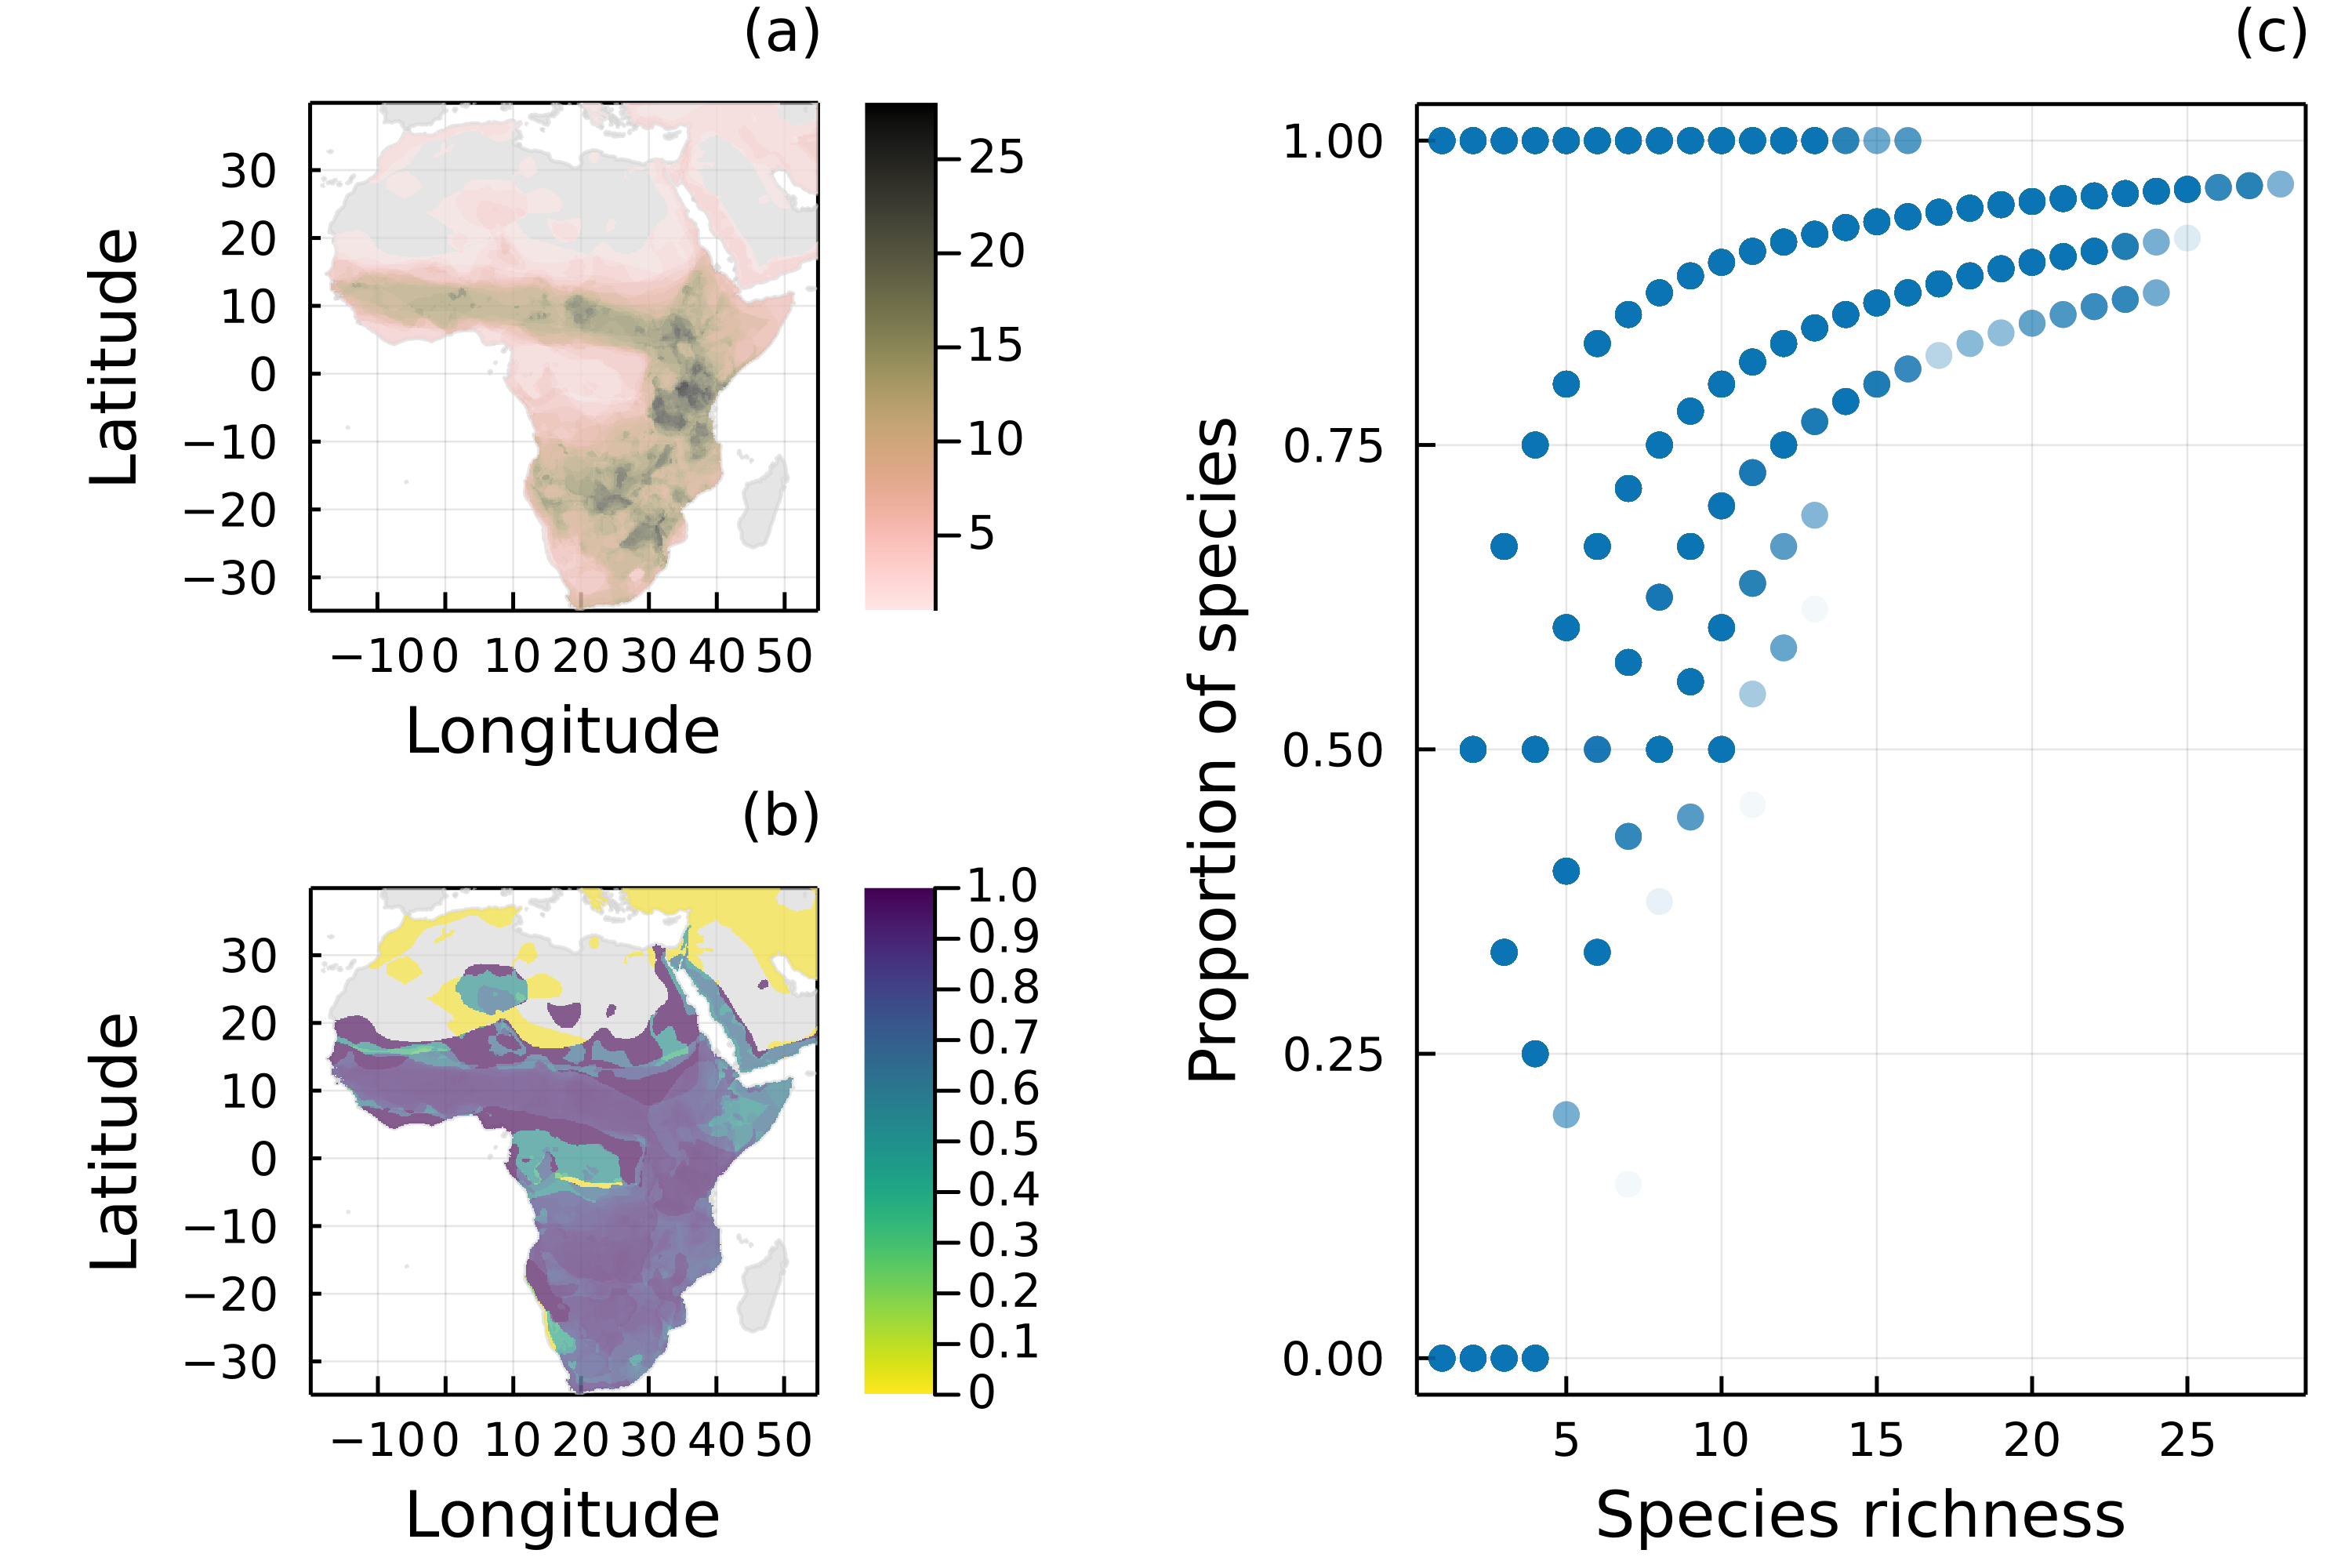
\includegraphics{figures/richness_prop_removed.png}
\caption{(a) Spatial distribution of species richness according to the
original IUCN range maps of all 32 mammal species of the Serengeti food
web. (b) Proportion of mammal species remaining in each local network
(i.e., each pixel) after removing all species without a path to a
primary producer. (c) Proportion of mammal species remaining in each
local network as a function of the number of species given by the
original IUCN range maps.}\label{fig:richness}
}
\end{figure}

\hypertarget{specialized-predators-have-higher-rates-of-range-mismatch}{%
\subsection{Specialized predators have higher rates of range
mismatch}\label{specialized-predators-have-higher-rates-of-range-mismatch}}

\begin{figure}
\hypertarget{fig:degree}{%
\centering
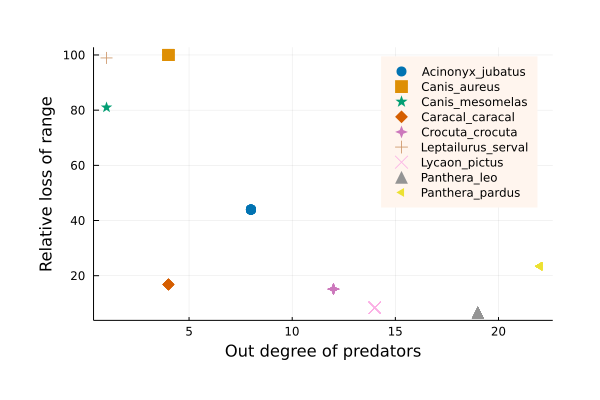
\includegraphics{figures/rel_loss-outdegree-species.png}
\caption{Negative relationship between the out degree of predator
species and their relative range mismatch. More specialized predators
``lose'' a higher proportion of their ranges due to mismatches with the
ranges of their preys.}\label{fig:degree}
}
\end{figure}

If we consider that we can not use areas where there are no
superposition between predators and prey on ecological analyses, we lose
more range area for predators with fewer prey (fig.~\ref{fig:degree}).
For instance, both \emph{Leptailurus serval} and \emph{Canis mesomelas}
have only one prey in the Serengeti food web (tbl.~\ref{tbl:everyone}),
each of them with a very small range compared to those of their
predator. This discrepancy between range sizes promotes significant
range loss. On the other hand, predators of the genus \emph{Panthera}
are some of the most connected species, and they also lose the least
proportion of their ranges. This mismatch between predators and preys
can also be a result of taxonomic disagreement between the geographical
and ecological data. Although \emph{Canis aureus} has the same number of
prey as \emph{Caracal caracal}, none of the prey taxa of the former
occurs inside its original range (tbl.~\ref{tbl:everyone}), which
results in complete range loss.

\begin{figure}
\hypertarget{fig:geo_diss}{%
\centering
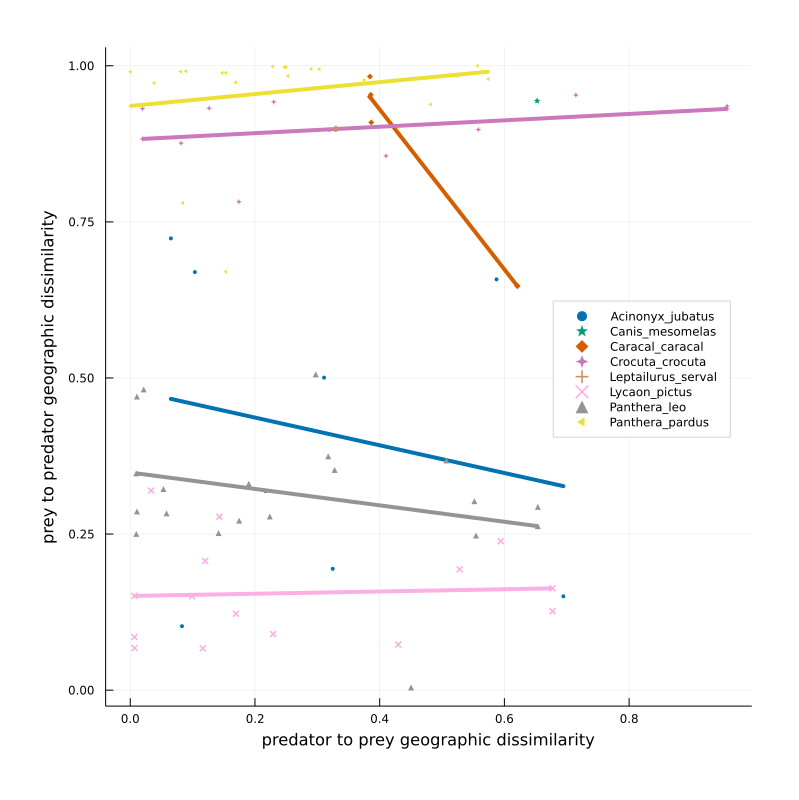
\includegraphics{figures/beta-div_pred-species.png}
\caption{Geographical similarity between the original IUCN range maps of
predators and preys. Dots represent predator-prey pairs, with different
symbols corresponding to different predators. For a given pair of
species, the number \(c\) of pixels where the focal species is present
but not the other and the number \(a\) of pixels where the predator and
prey cooccur, were calculated. Geographic similarities were given by
\(a/(a+c)\), with the predator being the focal species in the predator
to prey similarity (x-axis), while the prey is the focal one in the prey
to predator similarity (y-axis). One of the predators, \emph{Canis
aureus}, is not represented in the image because it is an extreme case
(where all its range is suppressed by the absence of preys) and it would
make the interpretation of the data more difficult.}\label{fig:geo_diss}
}
\end{figure}

There was a high variation in the overlap of predator and prey ranges
(fig.~\ref{fig:geo_diss}). The high density of points on the left-hand
side of fig.~\ref{fig:geo_diss} indicates that most preys have small
ranges in comparison to those of the set of carnivores in the networks,
resulting in either low overlap between both ranges (bottom) or high
overlap of ranges because much of that of the prey is within predators'
range (top). The top-right side of the plot encompasses situations where
the ranges of both predator and prey are similar and overlapping, while
the bottom-right part of the plot represents a situation where the range
of the predator is smaller than that of its prey and much of it occurs
within the preys' range. For example, \emph{Panthera pardus} had many
preys occurring inside its range, with highly variable levels of overlap
(tbl.~\ref{tbl:everyone}). In general, species exhibited more consistent
values of prey-predator overlap, than predator-prey overlap -- indicated
by the spread of points along the x-axis, yet more restricted variation
on the y-axis (fig.~\ref{fig:geo_diss}). There was also no overall
relationship between the two metrics, or for any predator species.

\hypertarget{tbl:everyone}{}
\begin{longtable}[]{@{}lrrrrr@{}}
\caption{\label{tbl:everyone}List of species analysed, their out and in
degrees, total original range size (in pixels), and proportion of their
ranges occupied by their preys and predators (values between 0 and 1).
Species are sorted according to the groups identified by Baskerville et
al. (2011). Notice how some species are isolated in the network
(\emph{Loxodonta africana}) and how \emph{Canis aureus}'s range does not
overlap with any of its preys.}\tabularnewline
\toprule
\begin{minipage}[b]{0.28\columnwidth}\raggedright
Species\strut
\end{minipage} & \begin{minipage}[b]{0.10\columnwidth}\raggedleft
Number of preys\strut
\end{minipage} & \begin{minipage}[b]{0.10\columnwidth}\raggedleft
Number of predators\strut
\end{minipage} & \begin{minipage}[b]{0.10\columnwidth}\raggedleft
Total range size\strut
\end{minipage} & \begin{minipage}[b]{0.13\columnwidth}\raggedleft
Proportion of range occupied by preys\strut
\end{minipage} & \begin{minipage}[b]{0.13\columnwidth}\raggedleft
Proportion of range occupied by predators\strut
\end{minipage}\tabularnewline
\midrule
\endfirsthead
\toprule
\begin{minipage}[b]{0.28\columnwidth}\raggedright
Species\strut
\end{minipage} & \begin{minipage}[b]{0.10\columnwidth}\raggedleft
Number of preys\strut
\end{minipage} & \begin{minipage}[b]{0.10\columnwidth}\raggedleft
Number of predators\strut
\end{minipage} & \begin{minipage}[b]{0.10\columnwidth}\raggedleft
Total range size\strut
\end{minipage} & \begin{minipage}[b]{0.13\columnwidth}\raggedleft
Proportion of range occupied by preys\strut
\end{minipage} & \begin{minipage}[b]{0.13\columnwidth}\raggedleft
Proportion of range occupied by predators\strut
\end{minipage}\tabularnewline
\midrule
\endhead
\begin{minipage}[t]{0.28\columnwidth}\raggedright
\textbf{Large carnivores}\strut
\end{minipage} & \begin{minipage}[t]{0.10\columnwidth}\raggedleft
\strut
\end{minipage} & \begin{minipage}[t]{0.10\columnwidth}\raggedleft
\strut
\end{minipage} & \begin{minipage}[t]{0.10\columnwidth}\raggedleft
\strut
\end{minipage} & \begin{minipage}[t]{0.13\columnwidth}\raggedleft
\strut
\end{minipage} & \begin{minipage}[t]{0.13\columnwidth}\raggedleft
\strut
\end{minipage}\tabularnewline
\begin{minipage}[t]{0.28\columnwidth}\raggedright
Acinonyx jubatus\strut
\end{minipage} & \begin{minipage}[t]{0.10\columnwidth}\raggedleft
8\strut
\end{minipage} & \begin{minipage}[t]{0.10\columnwidth}\raggedleft
1\strut
\end{minipage} & \begin{minipage}[t]{0.10\columnwidth}\raggedleft
9250\strut
\end{minipage} & \begin{minipage}[t]{0.13\columnwidth}\raggedleft
0.437\strut
\end{minipage} & \begin{minipage}[t]{0.13\columnwidth}\raggedleft
0.618\strut
\end{minipage}\tabularnewline
\begin{minipage}[t]{0.28\columnwidth}\raggedright
Crocuta crocuta\strut
\end{minipage} & \begin{minipage}[t]{0.10\columnwidth}\raggedleft
12\strut
\end{minipage} & \begin{minipage}[t]{0.10\columnwidth}\raggedleft
1\strut
\end{minipage} & \begin{minipage}[t]{0.10\columnwidth}\raggedleft
4822\strut
\end{minipage} & \begin{minipage}[t]{0.13\columnwidth}\raggedleft
0.844\strut
\end{minipage} & \begin{minipage}[t]{0.13\columnwidth}\raggedleft
0.253\strut
\end{minipage}\tabularnewline
\begin{minipage}[t]{0.28\columnwidth}\raggedright
Lycaon pictus\strut
\end{minipage} & \begin{minipage}[t]{0.10\columnwidth}\raggedleft
14\strut
\end{minipage} & \begin{minipage}[t]{0.10\columnwidth}\raggedleft
0\strut
\end{minipage} & \begin{minipage}[t]{0.10\columnwidth}\raggedleft
427\strut
\end{minipage} & \begin{minipage}[t]{0.13\columnwidth}\raggedleft
0.918\strut
\end{minipage} & \begin{minipage}[t]{0.13\columnwidth}\raggedleft
-\strut
\end{minipage}\tabularnewline
\begin{minipage}[t]{0.28\columnwidth}\raggedright
Panthera leo\strut
\end{minipage} & \begin{minipage}[t]{0.10\columnwidth}\raggedleft
18\strut
\end{minipage} & \begin{minipage}[t]{0.10\columnwidth}\raggedleft
0\strut
\end{minipage} & \begin{minipage}[t]{0.10\columnwidth}\raggedleft
1274\strut
\end{minipage} & \begin{minipage}[t]{0.13\columnwidth}\raggedleft
0.935\strut
\end{minipage} & \begin{minipage}[t]{0.13\columnwidth}\raggedleft
-\strut
\end{minipage}\tabularnewline
\begin{minipage}[t]{0.28\columnwidth}\raggedright
Panthera pardus\strut
\end{minipage} & \begin{minipage}[t]{0.10\columnwidth}\raggedleft
22\strut
\end{minipage} & \begin{minipage}[t]{0.10\columnwidth}\raggedleft
0\strut
\end{minipage} & \begin{minipage}[t]{0.10\columnwidth}\raggedleft
7563\strut
\end{minipage} & \begin{minipage}[t]{0.13\columnwidth}\raggedleft
0.766\strut
\end{minipage} & \begin{minipage}[t]{0.13\columnwidth}\raggedleft
-\strut
\end{minipage}\tabularnewline
\begin{minipage}[t]{0.28\columnwidth}\raggedright
\strut
\end{minipage} & \begin{minipage}[t]{0.10\columnwidth}\raggedleft
\strut
\end{minipage} & \begin{minipage}[t]{0.10\columnwidth}\raggedleft
\strut
\end{minipage} & \begin{minipage}[t]{0.10\columnwidth}\raggedleft
\strut
\end{minipage} & \begin{minipage}[t]{0.13\columnwidth}\raggedleft
\strut
\end{minipage} & \begin{minipage}[t]{0.13\columnwidth}\raggedleft
\strut
\end{minipage}\tabularnewline
\begin{minipage}[t]{0.28\columnwidth}\raggedright
\textbf{Small carnivores}\strut
\end{minipage} & \begin{minipage}[t]{0.10\columnwidth}\raggedleft
\strut
\end{minipage} & \begin{minipage}[t]{0.10\columnwidth}\raggedleft
\strut
\end{minipage} & \begin{minipage}[t]{0.10\columnwidth}\raggedleft
\strut
\end{minipage} & \begin{minipage}[t]{0.13\columnwidth}\raggedleft
\strut
\end{minipage} & \begin{minipage}[t]{0.13\columnwidth}\raggedleft
\strut
\end{minipage}\tabularnewline
\begin{minipage}[t]{0.28\columnwidth}\raggedright
Canis aureus\strut
\end{minipage} & \begin{minipage}[t]{0.10\columnwidth}\raggedleft
4\strut
\end{minipage} & \begin{minipage}[t]{0.10\columnwidth}\raggedleft
1\strut
\end{minipage} & \begin{minipage}[t]{0.10\columnwidth}\raggedleft
816\strut
\end{minipage} & \begin{minipage}[t]{0.13\columnwidth}\raggedleft
0.000\strut
\end{minipage} & \begin{minipage}[t]{0.13\columnwidth}\raggedleft
0.782\strut
\end{minipage}\tabularnewline
\begin{minipage}[t]{0.28\columnwidth}\raggedright
Canis mesomelas\strut
\end{minipage} & \begin{minipage}[t]{0.10\columnwidth}\raggedleft
1\strut
\end{minipage} & \begin{minipage}[t]{0.10\columnwidth}\raggedleft
1\strut
\end{minipage} & \begin{minipage}[t]{0.10\columnwidth}\raggedleft
2201\strut
\end{minipage} & \begin{minipage}[t]{0.13\columnwidth}\raggedleft
0.190\strut
\end{minipage} & \begin{minipage}[t]{0.13\columnwidth}\raggedleft
0.994\strut
\end{minipage}\tabularnewline
\begin{minipage}[t]{0.28\columnwidth}\raggedright
Caracal caracal\strut
\end{minipage} & \begin{minipage}[t]{0.10\columnwidth}\raggedleft
4\strut
\end{minipage} & \begin{minipage}[t]{0.10\columnwidth}\raggedleft
0\strut
\end{minipage} & \begin{minipage}[t]{0.10\columnwidth}\raggedleft
5239\strut
\end{minipage} & \begin{minipage}[t]{0.13\columnwidth}\raggedleft
0.833\strut
\end{minipage} & \begin{minipage}[t]{0.13\columnwidth}\raggedleft
-\strut
\end{minipage}\tabularnewline
\begin{minipage}[t]{0.28\columnwidth}\raggedright
Leptailurus serval\strut
\end{minipage} & \begin{minipage}[t]{0.10\columnwidth}\raggedleft
1\strut
\end{minipage} & \begin{minipage}[t]{0.10\columnwidth}\raggedleft
1\strut
\end{minipage} & \begin{minipage}[t]{0.10\columnwidth}\raggedleft
4319\strut
\end{minipage} & \begin{minipage}[t]{0.13\columnwidth}\raggedleft
0.011\strut
\end{minipage} & \begin{minipage}[t]{0.13\columnwidth}\raggedleft
0.978\strut
\end{minipage}\tabularnewline
\begin{minipage}[t]{0.28\columnwidth}\raggedright
\strut
\end{minipage} & \begin{minipage}[t]{0.10\columnwidth}\raggedleft
\strut
\end{minipage} & \begin{minipage}[t]{0.10\columnwidth}\raggedleft
\strut
\end{minipage} & \begin{minipage}[t]{0.10\columnwidth}\raggedleft
\strut
\end{minipage} & \begin{minipage}[t]{0.13\columnwidth}\raggedleft
\strut
\end{minipage} & \begin{minipage}[t]{0.13\columnwidth}\raggedleft
\strut
\end{minipage}\tabularnewline
\begin{minipage}[t]{0.28\columnwidth}\raggedright
\textbf{Small herbivores}\strut
\end{minipage} & \begin{minipage}[t]{0.10\columnwidth}\raggedleft
\strut
\end{minipage} & \begin{minipage}[t]{0.10\columnwidth}\raggedleft
\strut
\end{minipage} & \begin{minipage}[t]{0.10\columnwidth}\raggedleft
\strut
\end{minipage} & \begin{minipage}[t]{0.13\columnwidth}\raggedleft
\strut
\end{minipage} & \begin{minipage}[t]{0.13\columnwidth}\raggedleft
\strut
\end{minipage}\tabularnewline
\begin{minipage}[t]{0.28\columnwidth}\raggedright
Damaliscus lunatus\strut
\end{minipage} & \begin{minipage}[t]{0.10\columnwidth}\raggedleft
0\strut
\end{minipage} & \begin{minipage}[t]{0.10\columnwidth}\raggedleft
4\strut
\end{minipage} & \begin{minipage}[t]{0.10\columnwidth}\raggedleft
626\strut
\end{minipage} & \begin{minipage}[t]{0.13\columnwidth}\raggedleft
-\strut
\end{minipage} & \begin{minipage}[t]{0.13\columnwidth}\raggedleft
1\strut
\end{minipage}\tabularnewline
\begin{minipage}[t]{0.28\columnwidth}\raggedright
Hippopotamus amphibius\strut
\end{minipage} & \begin{minipage}[t]{0.10\columnwidth}\raggedleft
0\strut
\end{minipage} & \begin{minipage}[t]{0.10\columnwidth}\raggedleft
0\strut
\end{minipage} & \begin{minipage}[t]{0.10\columnwidth}\raggedleft
419\strut
\end{minipage} & \begin{minipage}[t]{0.13\columnwidth}\raggedleft
-\strut
\end{minipage} & \begin{minipage}[t]{0.13\columnwidth}\raggedleft
-\strut
\end{minipage}\tabularnewline
\begin{minipage}[t]{0.28\columnwidth}\raggedright
Kobus ellipsiprymnus\strut
\end{minipage} & \begin{minipage}[t]{0.10\columnwidth}\raggedleft
0\strut
\end{minipage} & \begin{minipage}[t]{0.10\columnwidth}\raggedleft
4\strut
\end{minipage} & \begin{minipage}[t]{0.10\columnwidth}\raggedleft
2961\strut
\end{minipage} & \begin{minipage}[t]{0.13\columnwidth}\raggedleft
-\strut
\end{minipage} & \begin{minipage}[t]{0.13\columnwidth}\raggedleft
1\strut
\end{minipage}\tabularnewline
\begin{minipage}[t]{0.28\columnwidth}\raggedright
Ourebia ourebi\strut
\end{minipage} & \begin{minipage}[t]{0.10\columnwidth}\raggedleft
0\strut
\end{minipage} & \begin{minipage}[t]{0.10\columnwidth}\raggedleft
5\strut
\end{minipage} & \begin{minipage}[t]{0.10\columnwidth}\raggedleft
2484\strut
\end{minipage} & \begin{minipage}[t]{0.13\columnwidth}\raggedleft
-\strut
\end{minipage} & \begin{minipage}[t]{0.13\columnwidth}\raggedleft
1\strut
\end{minipage}\tabularnewline
\begin{minipage}[t]{0.28\columnwidth}\raggedright
Pedetes capensis\strut
\end{minipage} & \begin{minipage}[t]{0.10\columnwidth}\raggedleft
0\strut
\end{minipage} & \begin{minipage}[t]{0.10\columnwidth}\raggedleft
2\strut
\end{minipage} & \begin{minipage}[t]{0.10\columnwidth}\raggedleft
1318\strut
\end{minipage} & \begin{minipage}[t]{0.13\columnwidth}\raggedleft
-\strut
\end{minipage} & \begin{minipage}[t]{0.13\columnwidth}\raggedleft
1\strut
\end{minipage}\tabularnewline
\begin{minipage}[t]{0.28\columnwidth}\raggedright
Phacochoerus africanus\strut
\end{minipage} & \begin{minipage}[t]{0.10\columnwidth}\raggedleft
0\strut
\end{minipage} & \begin{minipage}[t]{0.10\columnwidth}\raggedleft
5\strut
\end{minipage} & \begin{minipage}[t]{0.10\columnwidth}\raggedleft
3331\strut
\end{minipage} & \begin{minipage}[t]{0.13\columnwidth}\raggedleft
-\strut
\end{minipage} & \begin{minipage}[t]{0.13\columnwidth}\raggedleft
1\strut
\end{minipage}\tabularnewline
\begin{minipage}[t]{0.28\columnwidth}\raggedright
Redunca redunca\strut
\end{minipage} & \begin{minipage}[t]{0.10\columnwidth}\raggedleft
0\strut
\end{minipage} & \begin{minipage}[t]{0.10\columnwidth}\raggedleft
5\strut
\end{minipage} & \begin{minipage}[t]{0.10\columnwidth}\raggedleft
1935\strut
\end{minipage} & \begin{minipage}[t]{0.13\columnwidth}\raggedleft
-\strut
\end{minipage} & \begin{minipage}[t]{0.13\columnwidth}\raggedleft
1\strut
\end{minipage}\tabularnewline
\begin{minipage}[t]{0.28\columnwidth}\raggedright
Rhabdomys pumilio\strut
\end{minipage} & \begin{minipage}[t]{0.10\columnwidth}\raggedleft
0\strut
\end{minipage} & \begin{minipage}[t]{0.10\columnwidth}\raggedleft
5\strut
\end{minipage} & \begin{minipage}[t]{0.10\columnwidth}\raggedleft
53\strut
\end{minipage} & \begin{minipage}[t]{0.13\columnwidth}\raggedleft
-\strut
\end{minipage} & \begin{minipage}[t]{0.13\columnwidth}\raggedleft
1\strut
\end{minipage}\tabularnewline
\begin{minipage}[t]{0.28\columnwidth}\raggedright
Tragelaphus oryx\strut
\end{minipage} & \begin{minipage}[t]{0.10\columnwidth}\raggedleft
0\strut
\end{minipage} & \begin{minipage}[t]{0.10\columnwidth}\raggedleft
2\strut
\end{minipage} & \begin{minipage}[t]{0.10\columnwidth}\raggedleft
2316\strut
\end{minipage} & \begin{minipage}[t]{0.13\columnwidth}\raggedleft
-\strut
\end{minipage} & \begin{minipage}[t]{0.13\columnwidth}\raggedleft
0.990\strut
\end{minipage}\tabularnewline
\begin{minipage}[t]{0.28\columnwidth}\raggedright
Tragelaphus scriptus\strut
\end{minipage} & \begin{minipage}[t]{0.10\columnwidth}\raggedleft
0\strut
\end{minipage} & \begin{minipage}[t]{0.10\columnwidth}\raggedleft
3\strut
\end{minipage} & \begin{minipage}[t]{0.10\columnwidth}\raggedleft
3999\strut
\end{minipage} & \begin{minipage}[t]{0.13\columnwidth}\raggedleft
-\strut
\end{minipage} & \begin{minipage}[t]{0.13\columnwidth}\raggedleft
0.985\strut
\end{minipage}\tabularnewline
\begin{minipage}[t]{0.28\columnwidth}\raggedright
\strut
\end{minipage} & \begin{minipage}[t]{0.10\columnwidth}\raggedleft
\strut
\end{minipage} & \begin{minipage}[t]{0.10\columnwidth}\raggedleft
\strut
\end{minipage} & \begin{minipage}[t]{0.10\columnwidth}\raggedleft
\strut
\end{minipage} & \begin{minipage}[t]{0.13\columnwidth}\raggedleft
\strut
\end{minipage} & \begin{minipage}[t]{0.13\columnwidth}\raggedleft
\strut
\end{minipage}\tabularnewline
\begin{minipage}[t]{0.28\columnwidth}\raggedright
\textbf{Large grazers}\strut
\end{minipage} & \begin{minipage}[t]{0.10\columnwidth}\raggedleft
\strut
\end{minipage} & \begin{minipage}[t]{0.10\columnwidth}\raggedleft
\strut
\end{minipage} & \begin{minipage}[t]{0.10\columnwidth}\raggedleft
\strut
\end{minipage} & \begin{minipage}[t]{0.13\columnwidth}\raggedleft
\strut
\end{minipage} & \begin{minipage}[t]{0.13\columnwidth}\raggedleft
\strut
\end{minipage}\tabularnewline
\begin{minipage}[t]{0.28\columnwidth}\raggedright
Aepyceros melampus\strut
\end{minipage} & \begin{minipage}[t]{0.10\columnwidth}\raggedleft
0\strut
\end{minipage} & \begin{minipage}[t]{0.10\columnwidth}\raggedleft
5\strut
\end{minipage} & \begin{minipage}[t]{0.10\columnwidth}\raggedleft
1167\strut
\end{minipage} & \begin{minipage}[t]{0.13\columnwidth}\raggedleft
-\strut
\end{minipage} & \begin{minipage}[t]{0.13\columnwidth}\raggedleft
1\strut
\end{minipage}\tabularnewline
\begin{minipage}[t]{0.28\columnwidth}\raggedright
Alcelaphus buselaphus\strut
\end{minipage} & \begin{minipage}[t]{0.10\columnwidth}\raggedleft
0\strut
\end{minipage} & \begin{minipage}[t]{0.10\columnwidth}\raggedleft
4\strut
\end{minipage} & \begin{minipage}[t]{0.10\columnwidth}\raggedleft
2307\strut
\end{minipage} & \begin{minipage}[t]{0.13\columnwidth}\raggedleft
-\strut
\end{minipage} & \begin{minipage}[t]{0.13\columnwidth}\raggedleft
1\strut
\end{minipage}\tabularnewline
\begin{minipage}[t]{0.28\columnwidth}\raggedright
Connochaetes taurinus\strut
\end{minipage} & \begin{minipage}[t]{0.10\columnwidth}\raggedleft
0\strut
\end{minipage} & \begin{minipage}[t]{0.10\columnwidth}\raggedleft
6\strut
\end{minipage} & \begin{minipage}[t]{0.10\columnwidth}\raggedleft
1074\strut
\end{minipage} & \begin{minipage}[t]{0.13\columnwidth}\raggedleft
-\strut
\end{minipage} & \begin{minipage}[t]{0.13\columnwidth}\raggedleft
1\strut
\end{minipage}\tabularnewline
\begin{minipage}[t]{0.28\columnwidth}\raggedright
Equus quagga\strut
\end{minipage} & \begin{minipage}[t]{0.10\columnwidth}\raggedleft
0\strut
\end{minipage} & \begin{minipage}[t]{0.10\columnwidth}\raggedleft
5\strut
\end{minipage} & \begin{minipage}[t]{0.10\columnwidth}\raggedleft
786\strut
\end{minipage} & \begin{minipage}[t]{0.13\columnwidth}\raggedleft
-\strut
\end{minipage} & \begin{minipage}[t]{0.13\columnwidth}\raggedleft
1\strut
\end{minipage}\tabularnewline
\begin{minipage}[t]{0.28\columnwidth}\raggedright
Eudorcas thomsonii\strut
\end{minipage} & \begin{minipage}[t]{0.10\columnwidth}\raggedleft
0\strut
\end{minipage} & \begin{minipage}[t]{0.10\columnwidth}\raggedleft
6\strut
\end{minipage} & \begin{minipage}[t]{0.10\columnwidth}\raggedleft
51\strut
\end{minipage} & \begin{minipage}[t]{0.13\columnwidth}\raggedleft
-\strut
\end{minipage} & \begin{minipage}[t]{0.13\columnwidth}\raggedleft
1\strut
\end{minipage}\tabularnewline
\begin{minipage}[t]{0.28\columnwidth}\raggedright
Nanger granti\strut
\end{minipage} & \begin{minipage}[t]{0.10\columnwidth}\raggedleft
0\strut
\end{minipage} & \begin{minipage}[t]{0.10\columnwidth}\raggedleft
6\strut
\end{minipage} & \begin{minipage}[t]{0.10\columnwidth}\raggedleft
261\strut
\end{minipage} & \begin{minipage}[t]{0.13\columnwidth}\raggedleft
-\strut
\end{minipage} & \begin{minipage}[t]{0.13\columnwidth}\raggedleft
1\strut
\end{minipage}\tabularnewline
\begin{minipage}[t]{0.28\columnwidth}\raggedright
\strut
\end{minipage} & \begin{minipage}[t]{0.10\columnwidth}\raggedleft
\strut
\end{minipage} & \begin{minipage}[t]{0.10\columnwidth}\raggedleft
\strut
\end{minipage} & \begin{minipage}[t]{0.10\columnwidth}\raggedleft
\strut
\end{minipage} & \begin{minipage}[t]{0.13\columnwidth}\raggedleft
\strut
\end{minipage} & \begin{minipage}[t]{0.13\columnwidth}\raggedleft
\strut
\end{minipage}\tabularnewline
\begin{minipage}[t]{0.28\columnwidth}\raggedright
\textbf{Hyraxes}\strut
\end{minipage} & \begin{minipage}[t]{0.10\columnwidth}\raggedleft
\strut
\end{minipage} & \begin{minipage}[t]{0.10\columnwidth}\raggedleft
\strut
\end{minipage} & \begin{minipage}[t]{0.10\columnwidth}\raggedleft
\strut
\end{minipage} & \begin{minipage}[t]{0.13\columnwidth}\raggedleft
\strut
\end{minipage} & \begin{minipage}[t]{0.13\columnwidth}\raggedleft
\strut
\end{minipage}\tabularnewline
\begin{minipage}[t]{0.28\columnwidth}\raggedright
Heterohyrax brucei\strut
\end{minipage} & \begin{minipage}[t]{0.10\columnwidth}\raggedleft
0\strut
\end{minipage} & \begin{minipage}[t]{0.10\columnwidth}\raggedleft
1\strut
\end{minipage} & \begin{minipage}[t]{0.10\columnwidth}\raggedleft
1961\strut
\end{minipage} & \begin{minipage}[t]{0.13\columnwidth}\raggedleft
-\strut
\end{minipage} & \begin{minipage}[t]{0.13\columnwidth}\raggedleft
0.973\strut
\end{minipage}\tabularnewline
\begin{minipage}[t]{0.28\columnwidth}\raggedright
Procavia capensis\strut
\end{minipage} & \begin{minipage}[t]{0.10\columnwidth}\raggedleft
0\strut
\end{minipage} & \begin{minipage}[t]{0.10\columnwidth}\raggedleft
1\strut
\end{minipage} & \begin{minipage}[t]{0.10\columnwidth}\raggedleft
5312\strut
\end{minipage} & \begin{minipage}[t]{0.13\columnwidth}\raggedleft
-\strut
\end{minipage} & \begin{minipage}[t]{0.13\columnwidth}\raggedleft
0.647\strut
\end{minipage}\tabularnewline
\begin{minipage}[t]{0.28\columnwidth}\raggedright
\strut
\end{minipage} & \begin{minipage}[t]{0.10\columnwidth}\raggedleft
\strut
\end{minipage} & \begin{minipage}[t]{0.10\columnwidth}\raggedleft
\strut
\end{minipage} & \begin{minipage}[t]{0.10\columnwidth}\raggedleft
\strut
\end{minipage} & \begin{minipage}[t]{0.13\columnwidth}\raggedleft
\strut
\end{minipage} & \begin{minipage}[t]{0.13\columnwidth}\raggedleft
\strut
\end{minipage}\tabularnewline
\begin{minipage}[t]{0.28\columnwidth}\raggedright
\textbf{Others}\strut
\end{minipage} & \begin{minipage}[t]{0.10\columnwidth}\raggedleft
\strut
\end{minipage} & \begin{minipage}[t]{0.10\columnwidth}\raggedleft
\strut
\end{minipage} & \begin{minipage}[t]{0.10\columnwidth}\raggedleft
\strut
\end{minipage} & \begin{minipage}[t]{0.13\columnwidth}\raggedleft
\strut
\end{minipage} & \begin{minipage}[t]{0.13\columnwidth}\raggedleft
\strut
\end{minipage}\tabularnewline
\begin{minipage}[t]{0.28\columnwidth}\raggedright
Giraffa camelopardalis\strut
\end{minipage} & \begin{minipage}[t]{0.10\columnwidth}\raggedleft
0\strut
\end{minipage} & \begin{minipage}[t]{0.10\columnwidth}\raggedleft
1\strut
\end{minipage} & \begin{minipage}[t]{0.10\columnwidth}\raggedleft
607\strut
\end{minipage} & \begin{minipage}[t]{0.13\columnwidth}\raggedleft
-\strut
\end{minipage} & \begin{minipage}[t]{0.13\columnwidth}\raggedleft
0.473\strut
\end{minipage}\tabularnewline
\begin{minipage}[t]{0.28\columnwidth}\raggedright
Loxodonta africana\strut
\end{minipage} & \begin{minipage}[t]{0.10\columnwidth}\raggedleft
0\strut
\end{minipage} & \begin{minipage}[t]{0.10\columnwidth}\raggedleft
0\strut
\end{minipage} & \begin{minipage}[t]{0.10\columnwidth}\raggedleft
1078\strut
\end{minipage} & \begin{minipage}[t]{0.13\columnwidth}\raggedleft
-\strut
\end{minipage} & \begin{minipage}[t]{0.13\columnwidth}\raggedleft
-\strut
\end{minipage}\tabularnewline
\begin{minipage}[t]{0.28\columnwidth}\raggedright
Madoqua kirkii\strut
\end{minipage} & \begin{minipage}[t]{0.10\columnwidth}\raggedleft
0\strut
\end{minipage} & \begin{minipage}[t]{0.10\columnwidth}\raggedleft
7\strut
\end{minipage} & \begin{minipage}[t]{0.10\columnwidth}\raggedleft
443\strut
\end{minipage} & \begin{minipage}[t]{0.13\columnwidth}\raggedleft
-\strut
\end{minipage} & \begin{minipage}[t]{0.13\columnwidth}\raggedleft
1\strut
\end{minipage}\tabularnewline
\begin{minipage}[t]{0.28\columnwidth}\raggedright
Papio anubis\strut
\end{minipage} & \begin{minipage}[t]{0.10\columnwidth}\raggedleft
0\strut
\end{minipage} & \begin{minipage}[t]{0.10\columnwidth}\raggedleft
1\strut
\end{minipage} & \begin{minipage}[t]{0.10\columnwidth}\raggedleft
2571\strut
\end{minipage} & \begin{minipage}[t]{0.13\columnwidth}\raggedleft
-\strut
\end{minipage} & \begin{minipage}[t]{0.13\columnwidth}\raggedleft
0.937\strut
\end{minipage}\tabularnewline
\begin{minipage}[t]{0.28\columnwidth}\raggedright
Syncerus caffer\strut
\end{minipage} & \begin{minipage}[t]{0.10\columnwidth}\raggedleft
0\strut
\end{minipage} & \begin{minipage}[t]{0.10\columnwidth}\raggedleft
1\strut
\end{minipage} & \begin{minipage}[t]{0.10\columnwidth}\raggedleft
2808\strut
\end{minipage} & \begin{minipage}[t]{0.13\columnwidth}\raggedleft
-\strut
\end{minipage} & \begin{minipage}[t]{0.13\columnwidth}\raggedleft
0.251\strut
\end{minipage}\tabularnewline
\bottomrule
\end{longtable}

\hypertarget{validation-with-gbif-occurrences}{%
\subsection{Validation with GBIF
occurrences}\label{validation-with-gbif-occurrences}}

The proportion of GBIF pixels (pixels with at least one GBIF occurrence)
matching the IUCN ranges varied a lot for species with small ranges and
way less for species with large ranges (fig.~\ref{fig:gbif}, left). This
means that species with large ranges had more area where their datasets
for ecological and geographical information agreed. The lowest
proportions of GBIF pixels occurred for species with small ranges.
Amongst herbivores, \emph{Rhabdomys pumilio} has a proportion of 25.6\%
of its presence pixels within its IUCN range, while predators have this
proportion above 47\% (such as \emph{Lycaon pictus}, with 47.6\%, and
\emph{Panthera leo}, with 49.3\%). Nevertheless, some species with
smaller ranges showed high data overlap (such as \emph{Canis mesomelas},
with 94.1\%, and many herbivores). Overall, predators and preys
displayed similar overlap variations, and species with median and large
ranges had higher proportions of agreement between GBIF, IUCN and
interaction datasets.

The proportion of GBIF pixels in revised ranges can only be equal to or
lower than that of the original ranges, as our analysis removes pixels
from the original range and does not add new ones. Rather, the absence
of a difference between the two types of ranges indicates that no pixels
with GBIF observations, hence likely true habitats, were removed by our
analysis. Here this proportion was mostly similar to that of the
original IUCN ranges for most predator species (fig.~\ref{fig:gbif}).
Two species showed no difference in proportion (\emph{Lycaon pictus} and
\emph{Panthera leo}) while four species showed only small differences
(\emph{Crocuta crocuta} lost 0.4\% of the original data overlap;
\emph{Caracal caracal} lost 3.4\%; \emph{Acinonyx jubatus} and
\emph{Panthera pardus} lost 6.2\%). On the other hand, three species,
\emph{Canis aureus}, \emph{Canis mesomelas}, and \emph{Leptailurus
serval} showed very high differences, with overlaps lowered by 100\%,
58.4\%, and 100\% respectively. These last two species are also the only
predators with a single prey in our metaweb. \emph{Canis aureus} has
four preys, but it has one of the smallest ranges in IUCN, which is not
covered by any of its preys. This result reinforces the concern raised
in the literature on the use of IUCN range maps for species that are not
well known (Herkt, Skidmore, and Fahr 2017), demonstrating how small
range species are likely to have their distribution underestimated in
the IUCN database. Additionally, the fact that \emph{Canis aureus} had
such a conspicuous discrepancy between its original IUCN range and those
of its preys, and between GBIF and IUCN data, may indicate a taxonomic
incongruency between the three databases used here, which we explore in
the Discussion section. Our results delineate how a mismatch between
GBIF and IUCN databases differ greatly with small changes in herbivore
species ranges, and it is somewhat positively related to range size for
predator species. Moreover, we show that accounting for interactions
does not necessarily aggravates this dissimilarity, but it is relevant
for species about which we have little ecological information or for
specialists groups.

\begin{figure}
\hypertarget{fig:gbif}{%
\centering
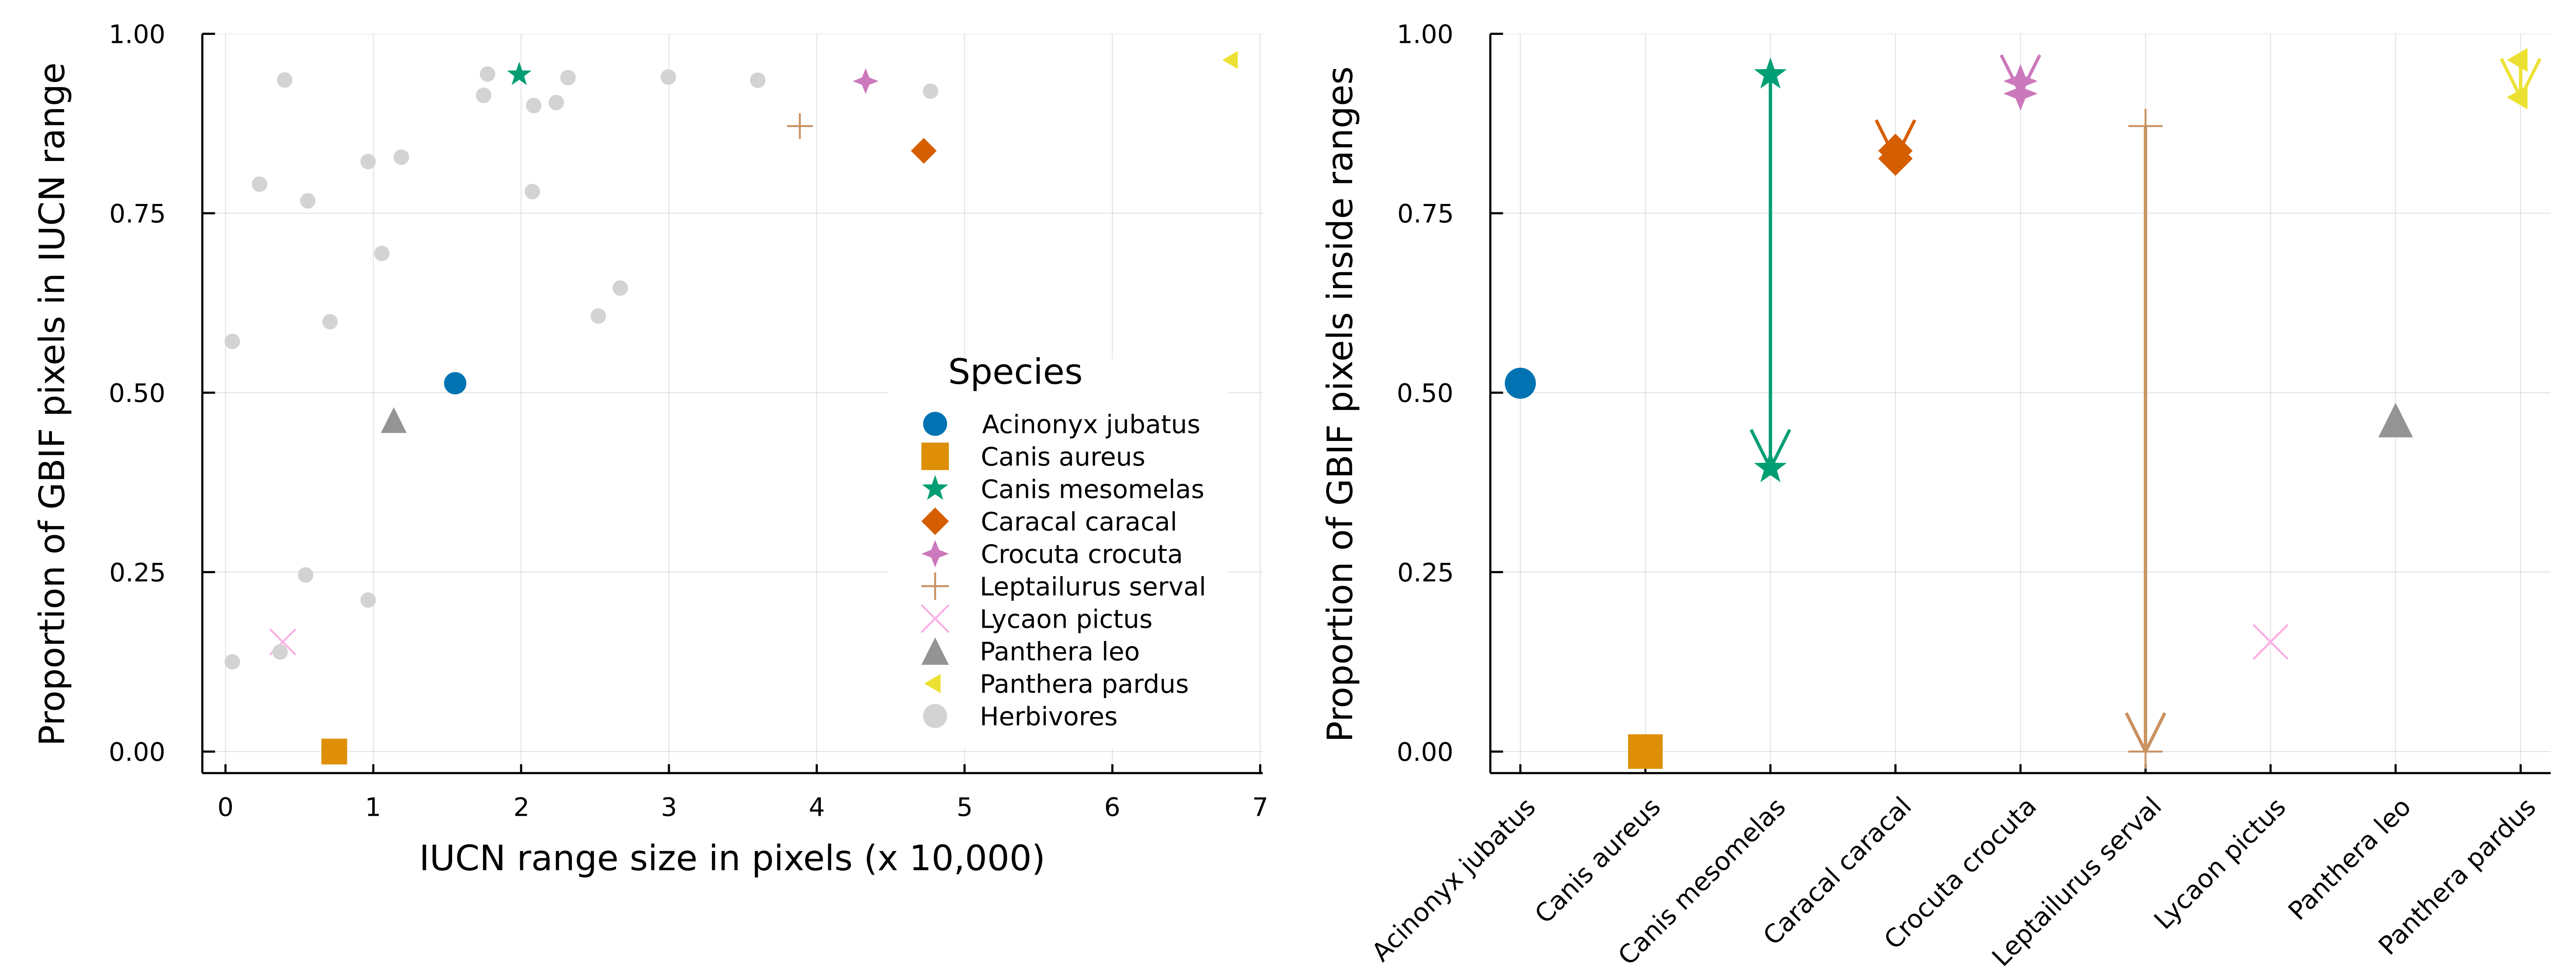
\includegraphics{figures/gbif_panels.png}
\caption{Left panel: Distribution of the proportion of GBIF pixels
(pixels with at least one occurrence in GBIF) supperposed by the IUCN
range data for different range sizes. Right panel: Differences between
the proportion of GBIF pixels matching the original and cropped IUCN
range maps for every predator species. Arrows go from the proportion
inside the original range to the proportion inside the revised range,
which can only be equal or lower. Overlapping markers indicate no
difference between the types of layers. Species markers are the same on
both figures, with predators presented in distinct colored markers and
all herbivores grouped in a single grey marker. Pixels represent a
resolution of 0.5 degrees.}\label{fig:gbif}
}
\end{figure}

\hypertarget{discussion}{%
\section{Discussion}\label{discussion}}

Here we identify areas of data mismatch between species range maps by
using ecological interaction data (predator-prey interactions within
food webs). Our results did show a significant mismatch in the IUCN
range areas of specialized and generalist predatory organisms and their
prey, which highlights the importance of accounting for species
interactions when estimating the range of a species. Although this type
of data mismatch can result of actual ecological processes, outdated
occurrence data, taxonomic errors and more, we argue that, here, they
rather indicate a lack of interaction sampling data.

The case of the golden jackal (\emph{Canis aureus}) is a good
illustration of how the taxonomic, geographical and ecological data can
be used to validate one another. The jackal is a widespread taxon in
northern Africa, Europe, and Australasia, generally well adapted to
local conditions due to its largely varied diet (Tsunoda and Saito 2020;
Krofel et al. 2021). Because of that, we expected that
the~\emph{Canis}~species in our dataset would be the ones losing the
least amount of range, with a higher value of the proportion of GBIF
pixels within their IUCN range maps. However, the taxonomy of this group
is a matter of intense discussion, as molecular and morphological data
seem to disagree in the clustering of species and subspecies (Krofel et
al. 2021; Stoyanov 2020). This debate probably influenced our results:
with originally only 64.9\% of the GBIF pixels of the golden jackal
overlapping with its IUCN data, we suspect that many of the GBIF
occurrences refer to other~\emph{Canis}~species, and that its taxonomic
identification in the network database is probably outdated. This led to
a complete exclusion of~\emph{Canis aureus}~from its original range in
our analysis, despite the fact that this species has four documented
preys in our metaweb.

\hypertarget{geographical-mismatch-and-data-availability}{%
\subsection{Geographical mismatch and data
availability}\label{geographical-mismatch-and-data-availability}}

The lack of superposition between IUCN range maps and GBIF occurrences
in our results suggests that we certainly miss geographical information
about the distribution of either the prey or the predator. On the other
hand, if both GBIF and IUCN occurrences tended to superpose and the
species was still locally removed, this indicates that we don't have
information about all its interactions (e.g., predators may be feeding
on different species than the ones in our dataset outside the Serengeti
ecosystem). This rationale can be illustrated with three types of
mismatches identified in our results.

First, \emph{Panthera leo} was one of the species with no difference
between ranges before and after our analysis, but 50.7\% of its IUCN
range map is not covered by the GBIF occurrences for this species, and
26.4\% of the GBIF point data does not overlap with its IUCN range map
(fig.~\ref{fig:gbif}). In this particular case, the IUCN maps seem to
agree with species interaction data. However, the disagreement between
the IUCN and the GBIF databases is concerning and suggests that the IUCN
maps might overestimate the lion's distribution.

On the other hand,~\emph{Leptailurus serval}~and~\emph{Canis
mesomelas}~are two of the three species that have the higher proportion
of mismatched range due to the lack of paths to a herbivore, but are
also some of the species with the higher proportion of GBIF occurrences
inside their original IUCN range maps (fig.~\ref{fig:gbif}). This
indicates that the information we are missing for these two species is
related to either an additional interaction or to the presence of
external interacting species. To illustrate that, we mapped the GBIF
data for the prey of~\emph{Leptailurus serval}, with a mobility buffer
around each point (fig.~\ref{fig:serval}). When considering GBIF data,
approximately 36\% of the prey's occurrences are within the portion of
the predator's range that was divergent from its original IUCN data.
With the buffer area, this corresponds to 5.57\% of the mismatched area.
By adding GBIF information for the prey, we could therefore reduce the
discrepancy of the range (or information) for the predator by 5.57\%
since its distribution is conditional on the occurrence of its preys. In
other words, the range mismatch was exagerated because we were missing
information on the presence of an interacting species (i.e., this also
indicates that there is a mismatch - or complementarity - between the
IUCN and GBIF data for their prey).

\begin{figure}
\hypertarget{fig:serval}{%
\centering
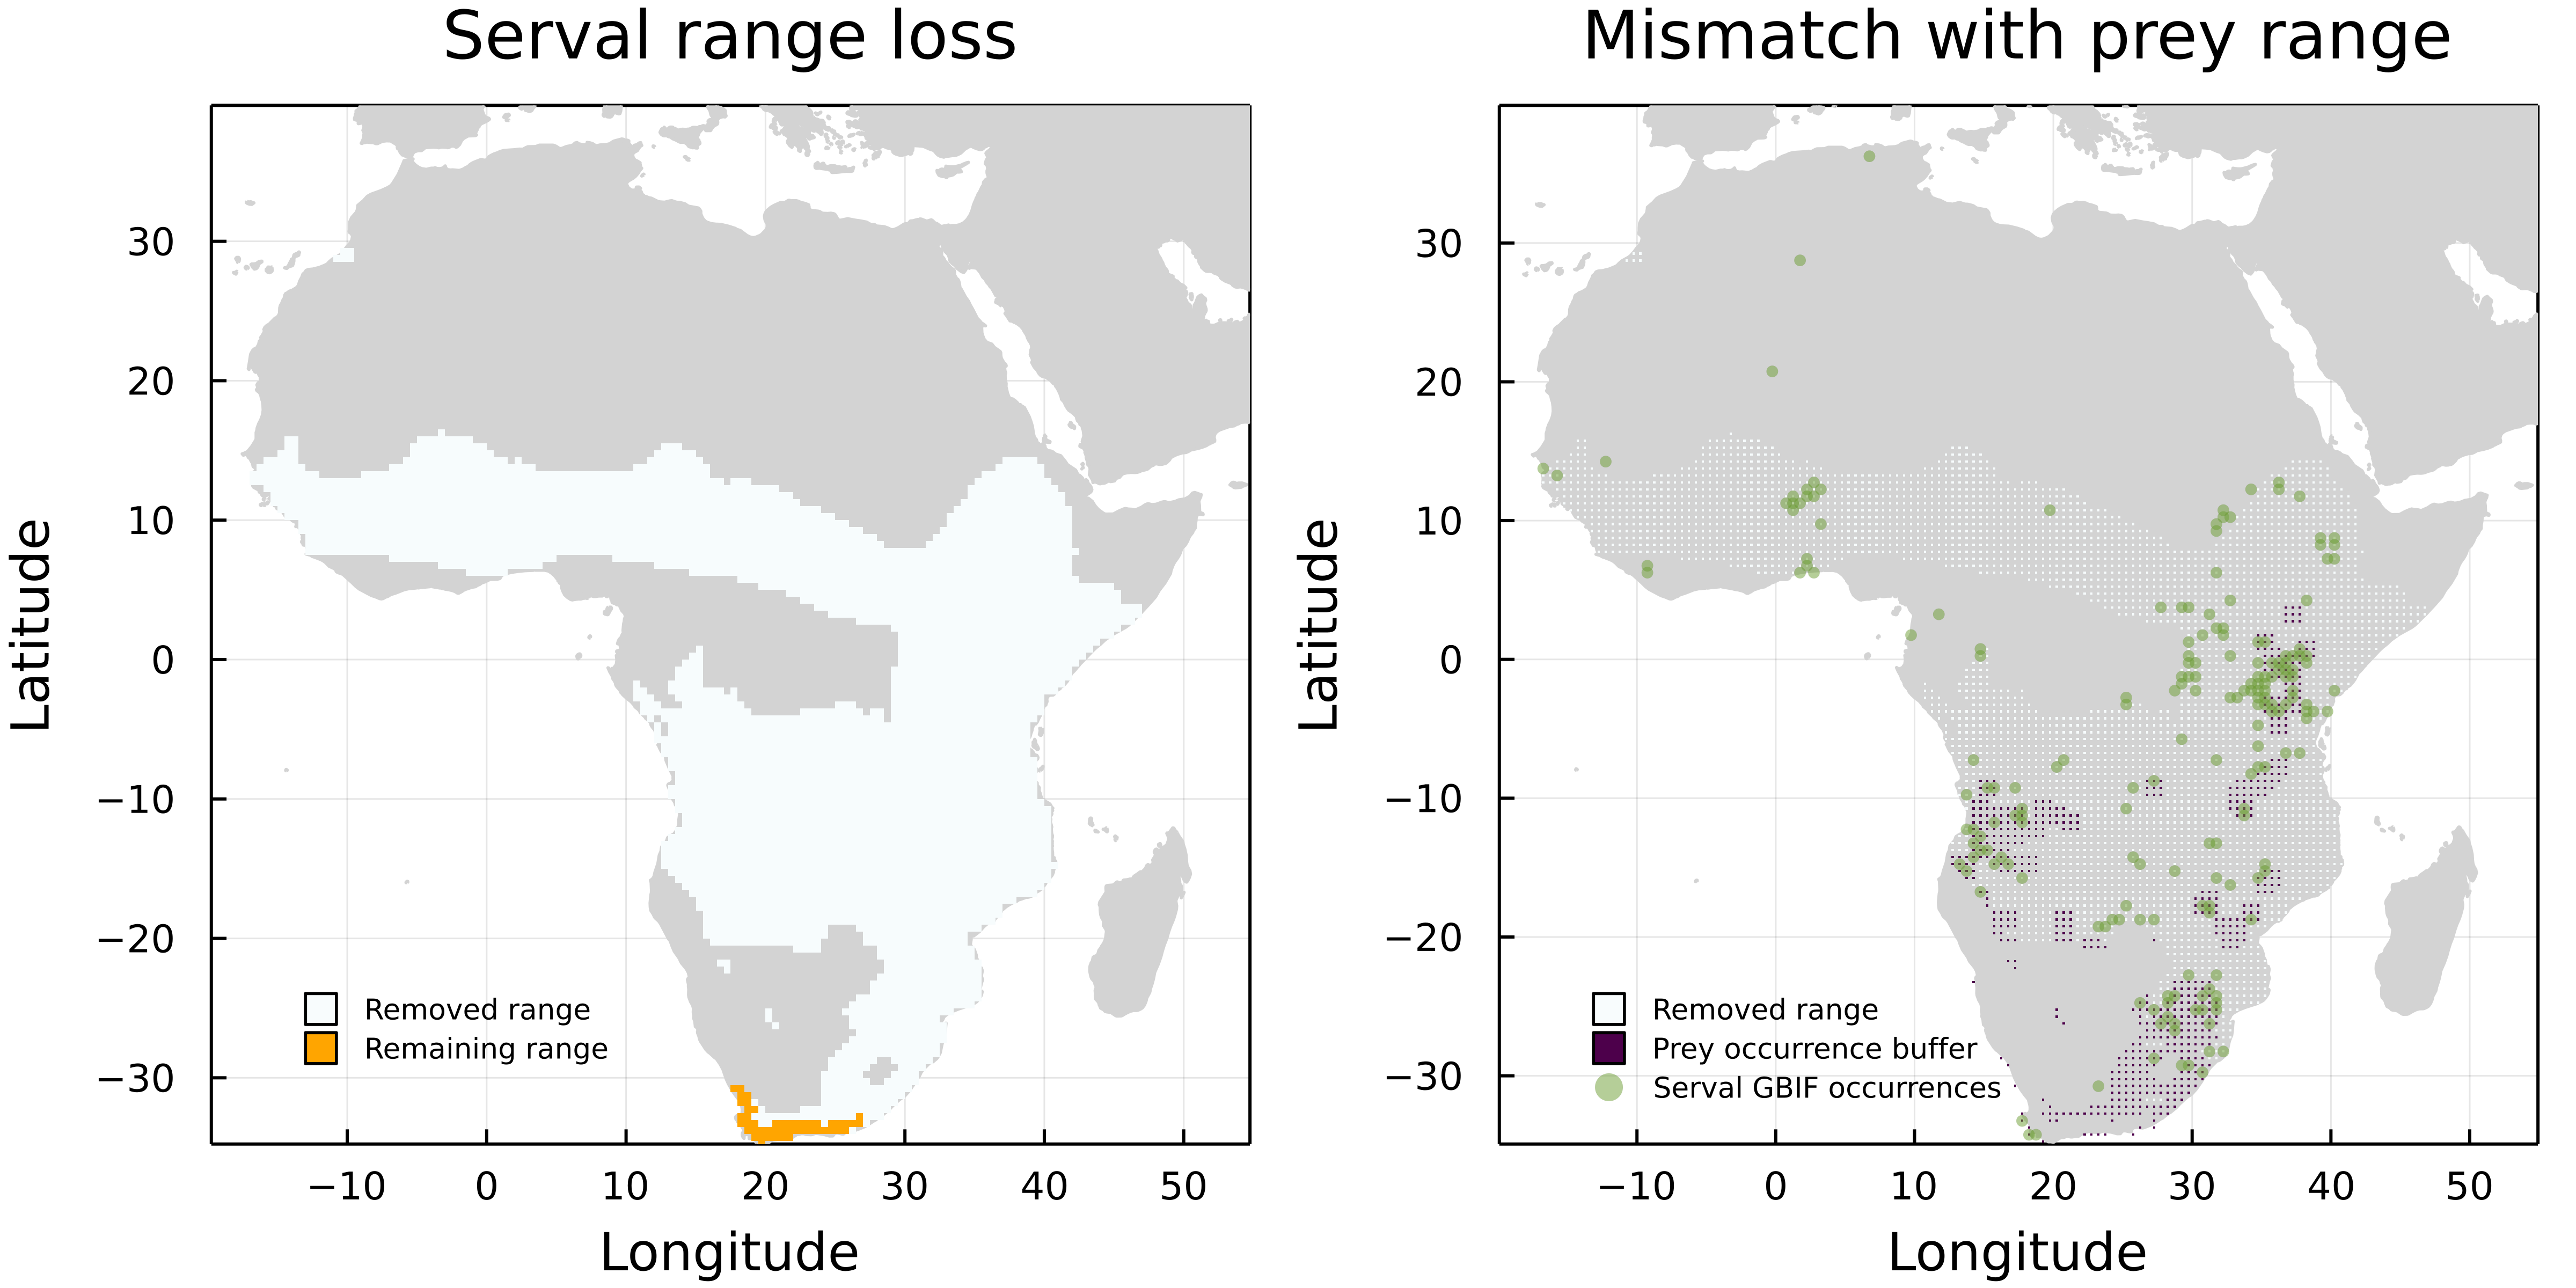
\includegraphics{figures/serval_mismatch_combined.png}
\caption{Mismatch between serval's range loss and GBIF occurrence of its
prey. The left panel shows the reduction of serval's range when we
consider the IUCN data on its prey. On the right panel, we added GBIF
data on both serval and its prey, with a buffer for the prey to account
for species mobility.}\label{fig:serval}
}
\end{figure}

Finally, the extreme case of~\emph{Canis aureus}~illustrates a lack of
both geographical and ecological information: only half of its GBIF
presence pixels and none of its preys occur inside its IUCN range. We
believe, therefore, that the validation of species distribution based on
ecological interaction is a relevant method that can further fill in
information gaps. Nevertheless, it is imperative that more
geographically explicit data about ecological networks and interactions
become available. This would help clarify when cooccurrences can be
translated into interactions (Windsor et al. 2022) and help the
development of more advanced validation methods for occurrence data.

\hypertarget{next-steps}{%
\subsection{Next steps}\label{next-steps}}

Here we demonstrated how we can detect areas of data deficit in species
distribution data using ecological interactions. Knowing where
questionable occurrence data are can be crucial in ecological modelling
(Hortal 2008; Ladle and Hortal 2013), and accounting for these errors
can improve model outputs by diminishing the error propagation (Draper
1995). For instance, we believe our method is a way to account for
ecological interactions in habitat suitability models without making the
models more complex, but by making sure (not assuming) that the input
data - the species occurrence - actually accounts for ecological
interactions. Another application of this method is mapping areas where
data are deficient and helping to indicate priority sampling locations
for interaction data, which can, in turn, reduce uncertainty in network
prediction. For example, if a certain pixel confirms the presence of a
species both with IUCN and GBIF data, but lacks connection between
species, this pixel has a high potential to hide an unobserved
interaction and should therefore be a priority sample location.\\
It is important to notice, however, that the quality and usefulness of
this method are highly correlated with the amount and quality of data
available about species' occurrences \textbf{and} interactions. With
this paper, we hope to add to the collective effort to decode the
encrypted message that is the occurrence of a species in space and time.
A promising avenue that adds to our method is the prediction of networks
and interactions in large scales (Strydom et al. 2021; Windsor et al.
2022), for they can add valuable information about ecological
interactions where they are missing. Additionally, in order to achieve a
robust modelling framework towards actual species distribution models we
should invest in efforts to collect and combine open data on species
occurrence and interactions (Windsor et al. 2022), especially because we
may be losing ecological interactions at least as fast as we are losing
species (Valiente-Banuet et al. 2015).

\hypertarget{acknowledgements}{%
\section{Acknowledgements}\label{acknowledgements}}

We acknowledge that this study was conducted on land within the
traditional unceded territory of the Saint Lawrence Iroquoian,
Anishinabewaki, Mohawk, Huron-Wendat, and Omàmiwininiwak nations. We
thank the editor and reviewers for their thoughtful comments, which
considerably improved this manuscript.

\hypertarget{references}{%
\section*{References}\label{references}}
\addcontentsline{toc}{section}{References}

\hypertarget{refs}{}
\begin{CSLReferences}{1}{0}
\leavevmode\hypertarget{ref-Abrego2021AccSpe}{}%
Abrego, Nerea, Tomas Roslin, Tea Huotari, Yinqiu Ji, Niels Martin
Schmidt, Jiaxin Wang, Douglas W. Yu, and Otso Ovaskainen. 2021.
{``Accounting for Species Interactions Is Necessary for Predicting How
Arctic Arthropod Communities Respond to Climate Change.''}
\emph{Ecography} 44 (6): 885--96.
\url{https://doi.org/10.1111/ecog.05547}.

\leavevmode\hypertarget{ref-Afkhami2014MutEff}{}%
Afkhami, Michelle E., Patrick J. McIntyre, and Sharon Y. Strauss. 2014.
{``Mutualist-Mediated Effects on Species' Range Limits Across Large
Geographic Scales.''} \emph{Ecology Letters} 17 (10): 1265--73.
\url{https://doi.org/10.1111/ele.12332}.

\leavevmode\hypertarget{ref-Albrecht2018PlaAni}{}%
Albrecht, Jörg. 2018. {``Plant and Animal Functional Diversity Drive
Mutualistic Network Assembly Across an Elevational Gradient.''}
\emph{NATURE COMMUNICATIONS}, 10.

\leavevmode\hypertarget{ref-Alhajeri2019HigCor}{}%
Alhajeri, Bader H, and Yoan Fourcade. 2019. {``High Correlation Between
Species-Level Environmental Data Estimates Extracted from IUCN Expert
Range Maps and from GBIF Occurrence Data.''} \emph{Journal of
Biogeography}, 13. \url{https://doi.org/10.1111/jbi.13619}.

\leavevmode\hypertarget{ref-Araujo2014ImpBio}{}%
Araújo, Carlos B. de, Luiz Octavio Marcondes-Machado, and Gabriel C.
Costa. 2014. {``The Importance of Biotic Interactions in Species
Distribution Models: A Test of the Eltonian Noise Hypothesis Using
Parrots.''} \emph{Journal of Biogeography} 41 (3): 513--23.
\url{https://doi.org/10.1111/jbi.12234}.

\leavevmode\hypertarget{ref-Baskerville2011SpaGui}{}%
Baskerville, Edward B., Andy P. Dobson, Trevor Bedford, Stefano
Allesina, T. Michael Anderson, and Mercedes Pascual. 2011. {``Spatial
Guilds in the Serengeti Food Web Revealed by a Bayesian Group Model.''}
\emph{PLOS Computational Biology} 7 (12): e1002321.
\url{https://doi.org/10.1371/journal.pcbi.1002321}.

\leavevmode\hypertarget{ref-Bezanson2017JulFre}{}%
Bezanson, Jeff, Alan Edelman, Stefan Karpinski, and Viral B. Shah. 2017.
{``Julia: A Fresh Approach to Numerical Computing.''} \emph{SIAM Review}
59 (1): 65--98. \url{https://doi.org/10.1137/141000671}.

\leavevmode\hypertarget{ref-Blanchet2020CooNot}{}%
Blanchet, F. Guillaume, Kevin Cazelles, and Dominique Gravel. 2020.
{``Co-Occurrence Is Not Evidence of Ecological Interactions.''}
\emph{Ecology Letters} 23 (7): 1050--63.
\url{https://doi.org/10.1111/ele.13525}.

\leavevmode\hypertarget{ref-Boakes2010DisVie}{}%
Boakes, Elizabeth H., Philip J. K. McGowan, Richard A. Fuller, Ding
Chang-qing, Natalie E. Clark, Kim O'Connor, and Georgina M. Mace. 2010.
{``Distorted Views of Biodiversity: Spatial and Temporal Bias in Species
Occurrence Data.''} \emph{PLOS Biology} 8 (6): e1000385.
\url{https://doi.org/10.1371/journal.pbio.1000385}.

\leavevmode\hypertarget{ref-Cabral2017MecSim}{}%
Cabral, Juliano Sarmento, Luis Valente, and Florian Hartig. 2017.
{``Mechanistic Simulation Models in Macroecology and Biogeography:
State-of-Art and Prospects.''} \emph{Ecography} 40 (2): 267--80.
\url{https://doi.org/10.1111/ecog.02480}.

\leavevmode\hypertarget{ref-Callaghan2019ImpBig}{}%
Callaghan, Corey T., Jodi J. L. Rowley, William K. Cornwell, Alistair G.
B. Poore, and Richard E. Major. 2019. {``Improving Big Citizen Science
Data: Moving Beyond Haphazard Sampling.''} \emph{PLOS Biology} 17 (6):
e3000357. \url{https://doi.org/10.1371/journal.pbio.3000357}.

\leavevmode\hypertarget{ref-Dallas2020AbuNot}{}%
Dallas, Tad, Samuel Pironon, and Luca Santini. 2020. {``The
Abundant-Centre Is Not All That Abundant: A Comment to Osorio-Olvera Et
Al. 2020,''} 2020.02.27.968586.
\url{https://doi.org/10.1101/2020.02.27.968586}.

\leavevmode\hypertarget{ref-Dansereau2021SimJl}{}%
Dansereau, Gabriel, and Timothée Poisot. 2021. {``SimpleSDMLayers.jl and
GBIF.jl: A Framework for Species Distribution Modeling in Julia.''}
\emph{Journal of Open Source Software} 6 (57): 2872.
\url{https://doi.org/10.21105/joss.02872}.

\leavevmode\hypertarget{ref-Daru2020GreToo}{}%
Daru, Barnabas H. 2020. {``GreenMaps: A Tool for Addressing the
Wallacean Shortfall in the Global Distribution of Plants.''}
\emph{bioRxiv}, 2020.02.21.960161.
\url{https://doi.org/10.1101/2020.02.21.960161}.

\leavevmode\hypertarget{ref-Dobson2009FooStr}{}%
Dobson, Andy. 2009. {``Food-Web Structure and Ecosystem Services:
Insights from the Serengeti.''} \emph{Philosophical Transactions of the
Royal Society B: Biological Sciences} 364 (1524): 1665--82.
\url{https://doi.org/10.1098/rstb.2008.0287}.

\leavevmode\hypertarget{ref-Draper1995AssPro}{}%
Draper, D. 1995. {``Assessment and Propagation of Model Uncertainty.''}
\emph{Journal of the Royal Statistical Society Series B-Statistical
Methodology} 57 (1): 45--97.
\url{https://doi.org/10.1111/j.2517-6161.1995.tb02015.x}.

\leavevmode\hypertarget{ref-Ficetola2014EvaRob}{}%
Ficetola, Gentile Francesco, Carlo Rondinini, Anna Bonardi, Vineet
Katariya, Emilio Padoa-Schioppa, and Ariadne Angulo. 2014. {``An
Evaluation of the Robustness of Global Amphibian Range Maps.''}
\emph{Journal of Biogeography} 41 (2): 211--21.
\url{https://doi.org/10.1111/jbi.12206}.

\leavevmode\hypertarget{ref-Fourcade2016ComSpe}{}%
Fourcade, Yoan. 2016. {``Comparing Species Distributions Modelled from
Occurrence Data and from Expert-Based Range Maps. Implication for
Predicting Range Shifts with Climate Change.''} \emph{Ecological
Informatics} 36: 8--14.
\url{https://doi.org/10.1016/j.ecoinf.2016.09.002}.

\leavevmode\hypertarget{ref-Fricke2022EffDef}{}%
Fricke, Evan C., Alejandro Ordonez, Haldre S. Rogers, and Jens-Christian
Svenning. 2022. {``The Effects of Defaunation on Plants' Capacity to
Track Climate Change.''} \emph{Science}.
\url{https://doi.org/10.1126/science.abk3510}.

\leavevmode\hypertarget{ref-GBIF.org2022GbiOcc}{}%
GBIF.org. 2022. {``GBIF Occurrence Download.''} The Global Biodiversity
Information Facility. \url{https://doi.org/10.15468/DL.PF4586}.

\leavevmode\hypertarget{ref-GBIFSecretariat2021GbiBac}{}%
GBIF Secretariat. 2021. {``GBIF Backbone Taxonomy.''}
\url{https://doi.org/10.15468/39omei}.

\leavevmode\hypertarget{ref-GDALux2fOGRcontributors2021GdaOgr}{}%
GDAL/OGR contributors. 2021. \emph{GDAL/OGR Geospatial Data Abstraction
Software Library}. Manual. Open Source Geospatial Foundation.

\leavevmode\hypertarget{ref-Godsoe2012HowSpe}{}%
Godsoe, William, and Luke J. Harmon. 2012. {``How Do Species
Interactions Affect Species Distribution Models?''} \emph{Ecography} 35
(9): 811--20. \url{https://doi.org/10.1111/j.1600-0587.2011.07103.x}.

\leavevmode\hypertarget{ref-Godsoe2017IntBio}{}%
Godsoe, William, Jill Jankowski, Robert D. Holt, and Dominique Gravel.
2017. {``Integrating Biogeography with Contemporary Niche Theory.''}
\emph{Trends in Ecology and Evolution} 32 (7): 488--99.
\url{https://doi.org/10.1016/j.tree.2017.03.008}.

\leavevmode\hypertarget{ref-Gotelli2010MacSig}{}%
Gotelli, Nicholas J., Gary R. Graves, and Carsten Rahbek. 2010.
{``Macroecological Signals of Species Interactions in the Danish
Avifauna.''} \emph{Proceedings of the National Academy of Sciences} 107
(11): 5030--35. \url{https://doi.org/10.1073/pnas.0914089107}.

\leavevmode\hypertarget{ref-Herkt2017MacCon}{}%
Herkt, K. Matthias B., Andrew K. Skidmore, and Jakob Fahr. 2017.
{``Macroecological Conclusions Based on IUCN Expert Maps: A Call for
Caution.''} \emph{Global Ecology and Biogeography} 26 (8): 930--41.
\url{https://doi.org/10.1111/geb.12601}.

\leavevmode\hypertarget{ref-Hortal2008UncMea}{}%
Hortal, Joaquín. 2008. {``Uncertainty and the Measurement of Terrestrial
Biodiversity Gradients.''} \emph{Journal of Biogeography} 35 (8):
1335--36. \url{https://doi.org/10.1111/j.1365-2699.2008.01955.x}.

\leavevmode\hypertarget{ref-Hortal2015SevSho}{}%
Hortal, Joaquín, Francesco de Bello, José Alexandre F. Diniz-Filho,
Thomas M. Lewinsohn, Jorge M. Lobo, and Richard J. Ladle. 2015. {``Seven
Shortfalls That Beset Large-Scale Knowledge of Biodiversity.''}
\emph{Annual Review of Ecology, Evolution, and Systematics} 46 (1):
523--49. \url{https://doi.org/10.1146/annurev-ecolsys-112414-054400}.

\leavevmode\hypertarget{ref-Hortal2008HisBia}{}%
Hortal, Joaquín, Alberto Jiménez-Valverde, José F. Gómez, Jorge M. Lobo,
and Andrés Baselga. 2008. {``Historical Bias in Biodiversity Inventories
Affects the Observed Environmental Niche of the Species.''} \emph{Oikos}
117 (6): 847--58.
\url{https://doi.org/10.1111/j.0030-1299.2008.16434.x}.

\leavevmode\hypertarget{ref-Hurlbert2007SpeRic}{}%
Hurlbert, Allen H., and Walter Jetz. 2007. {``Species Richness,
Hotspots, and the Scale Dependence of Range Maps in Ecology and
Conservation.''} \emph{Proceedings of the National Academy of Sciences}
104 (33): 13384--89. \url{https://doi.org/10.1073/pnas.0704469104}.

\leavevmode\hypertarget{ref-Hurlbert2005DisRan}{}%
Hurlbert, Allen H., and Ethan P. White. 2005. {``Disparity Between Range
Map- and Survey-Based Analyses of Species Richness: Patterns, Processes
and Implications.''} \emph{Ecology Letters} 8 (3): 319--27.
\url{https://doi.org/10.1111/j.1461-0248.2005.00726.x}.

\leavevmode\hypertarget{ref-Isaac2004TaxInf}{}%
Isaac, Nick J. B., James Mallet, and Georgina M. Mace. 2004.
{``Taxonomic Inflation: Its Influence on Macroecology and
Conservation.''} \emph{Trends in Ecology \& Evolution} 19 (9): 464--69.
\url{https://doi.org/10.1016/j.tree.2004.06.004}.

\leavevmode\hypertarget{ref-IUCN2019MapSta}{}%
IUCN Red List Technical Working Group. 2019. {``Mapping Standards and
Data Quality for IUCN Red List Spatial Data.''} Prepared by the
Standards and Petitions Working Group of the IUCN SSC Red \ldots.

\leavevmode\hypertarget{ref-Krofel2021ResTax}{}%
Krofel, M., J. Hatlauf, W. Bogdanowicz, L. a. D. Campbell, R. Godinho,
Y. V. Jhala, A. C. Kitchener, et al. 2021. {``Towards Resolving
Taxonomic Uncertainties in Wolf, Dog and Jackal Lineages of Africa,
Eurasia and Australasia.''} \emph{Journal of Zoology} n/a (n/a): 1--14.
\url{https://doi.org/10.1111/jzo.12946}.

\leavevmode\hypertarget{ref-Ladle2013MapSpe}{}%
Ladle, Richard, and Joaquín Hortal. 2013. {``Mapping Species
Distributions: Living with Uncertainty.''} \emph{Frontiers of
Biogeography} 5 (1): 4--6.

\leavevmode\hypertarget{ref-McNaughton1992ProDis}{}%
McNaughton, S. J. 1992. {``The Propagation of Disturbance in Savannas
Through Food Webs.''} \emph{Journal of Vegetation Science} 3 (3):
301--14. \url{https://doi.org/10.2307/3235755}.

\leavevmode\hypertarget{ref-Meyer2016MulBia}{}%
Meyer, Carsten, Patrick Weigelt, and Holger Kreft. 2016.
{``Multidimensional Biases, Gaps and Uncertainties in Global Plant
Occurrence Information.''} \emph{Ecology Letters} 19 (8): 992--1006.
\url{https://doi.org/10.1111/ele.12624}.

\leavevmode\hypertarget{ref-Pocock2015BioRec}{}%
Pocock, Michael J. O., Helen E. Roy, Chris D. Preston, and David B. Roy.
2015. {``The Biological Records Centre: A Pioneer of Citizen Science.''}
\emph{Biological Journal of the Linnean Society} 115 (3): 475--93.
\url{https://doi.org/10.1111/bij.12548}.

\leavevmode\hypertarget{ref-Poisot2016ManMak}{}%
Poisot, Timothée, Benjamin Baiser, Jennifer A Dunne, Sonia Kéfi,
François Massol, Nicolas Mouquet, Tamara N Romanuk, Daniel B Stouffer,
Spencer A Wood, and Dominique Gravel. 2016. {``Mangal - Making
Ecological Network Analysis Simple.''} \emph{Ecography} 39 (4): 384--90.

\leavevmode\hypertarget{ref-Poisot2021GloKno}{}%
Poisot, Timothée, Gabriel Bergeron, Kevin Cazelles, Tad Dallas,
Dominique Gravel, Andrew MacDonald, Benjamin Mercier, Clément Violet,
and Steve Vissault. 2021. {``Global Knowledge Gaps in Species
Interaction Networks Data.''} \emph{Journal of Biogeography} 48 (7):
1552--63. \url{https://doi.org/10.1111/jbi.14127}.

\leavevmode\hypertarget{ref-Poisot2020EnvBia}{}%
Poisot, Timothée, Gabriel Bergeron, Kevin Cazelles, Tad Dallas,
Dominique Gravel, Andrew Macdonald, Benjamin Mercier, Clément Violet,
and Steve Vissault. 2020. {``Environmental Biases in the Study of
Ecological Networks at the Planetary Scale.''} \emph{bioRxiv},
2020.01.27.921429. \url{https://doi.org/10.1101/2020.01.27.921429}.

\leavevmode\hypertarget{ref-Poisot2019EcoJl}{}%
Poisot, Timothée, Zachary Bélisle, Laura Hoebeke, Michiel Stock, and
Piotr Szefer. 2019. {``EcologicalNetworks.jl: Analysing Ecological
Networks of Species Interactions.''} \emph{Ecography} 42 (11): 1850--61.
\url{https://doi.org/10.1111/ecog.04310}.

\leavevmode\hypertarget{ref-Power1992TopBot}{}%
Power, Mary E. 1992. {``Top-Down and Bottom-Up Forces in Food Webs: Do
Plants Have Primacy.''} \emph{Ecology} 73 (3): 733--46.
\url{https://doi.org/10.2307/1940153}.

\leavevmode\hypertarget{ref-Rondinini2006TraDif}{}%
Rondinini, Carlo, Kerrie A. Wilson, Luigi Boitani, Hedley Grantham, and
Hugh P. Possingham. 2006. {``Tradeoffs of Different Types of Species
Occurrence Data for Use in Systematic Conservation Planning.''}
\emph{Ecology Letters} 9 (10): 1136--45.
\url{https://doi.org/10.1111/j.1461-0248.2006.00970.x}.

\leavevmode\hypertarget{ref-Ronquillo2020AssSpa}{}%
Ronquillo, Cristina, Fernanda Alves-Martins, Vicente Mazimpaka, Thadeu
Sobral-Souza, Bruno Vilela-Silva, Nagore G. Medina, and Joaquín Hortal.
2020. {``Assessing Spatial and Temporal Biases and Gaps in the Publicly
Available Distributional Information of Iberian Mosses.''}
\emph{Biodiversity Data Journal} 8: e53474.
\url{https://doi.org/10.3897/BDJ.8.e53474}.

\leavevmode\hypertarget{ref-Roy2016FocPla}{}%
Roy, Helen E., Elizabeth Baxter, Aoine Saunders, and Michael J. O.
Pocock. 2016. {``Focal Plant Observations as a Standardised Method for
Pollinator Monitoring: Opportunities and Limitations for Mass
Participation Citizen Science.''} \emph{PLOS ONE} 11 (3): e0150794.
\url{https://doi.org/10.1371/journal.pone.0150794}.

\leavevmode\hypertarget{ref-Ryan2018RolCit}{}%
Ryan, S. F., N. L. Adamson, A. Aktipis, L. K. Andersen, R. Austin, L.
Barnes, M. R. Beasley, et al. 2018. {``The Role of Citizen Science in
Addressing Grand Challenges in Food and Agriculture Research.''}
\emph{Proceedings of the Royal Society B: Biological Sciences} 285
(1891). \url{https://doi.org/10.1098/rspb.2018.1977}.

\leavevmode\hypertarget{ref-Scott2018RolHer}{}%
Scott, Abigail L., Paul H. York, Clare Duncan, Peter I. Macreadie, Rod
M. Connolly, Megan T. Ellis, Jessie C. Jarvis, Kristin I. Jinks, Helene
Marsh, and Michael A. Rasheed. 2018. {``The Role of Herbivory in
Structuring Tropical Seagrass Ecosystem Service Delivery.''}
\emph{Frontiers in Plant Science} 9: 127.
\url{https://doi.org/10.3389/fpls.2018.00127}.

\leavevmode\hypertarget{ref-Stoyanov2020CraVar}{}%
Stoyanov, S. 2020. {``Cranial Variability and Differentiation Among
Golden Jackals (Canis Aureus) in Europe, Asia Minor and Africa.''}
\emph{ZooKeys}. \url{https://doi.org/10.3897/zookeys.917.39449}.

\leavevmode\hypertarget{ref-Strydom2021RoaPre}{}%
Strydom, Tanya, Michael D. Catchen, Francis Banville, Dominique Caron,
Gabriel Dansereau, Philippe Desjardins-Proulx, Norma R. Forero-Muñoz, et
al. 2021. {``A Roadmap Towards Predicting Species Interaction Networks
(across Space and Time).''} \emph{Philosophical Transactions of the
Royal Society B: Biological Sciences} 376 (1837): 20210063.
\url{https://doi.org/10.1098/rstb.2021.0063}.

\leavevmode\hypertarget{ref-Tsunoda2020VarTro}{}%
Tsunoda, Hiroshi, and Masayuki U. Saito. 2020. {``Variations in the
Trophic Niches of the Golden Jackal Canis Aureus Across the Eurasian
Continent Associated with Biogeographic and Anthropogenic Factors.''}
\emph{Journal of Vertebrate Biology} 69 (4): 20056.1.
\url{https://doi.org/10.25225/jvb.20056}.

\leavevmode\hypertarget{ref-Valiente-Banuet2015SpeLos}{}%
Valiente-Banuet, Alfonso, Marcelo A. Aizen, Julio M. Alcántara, Juan
Arroyo, Andrea Cocucci, Mauro Galetti, María B. García, et al. 2015.
{``Beyond Species Loss: The Extinction of Ecological Interactions in a
Changing World.''} Edited by Marc Johnson. \emph{Functional Ecology} 29
(3): 299--307. \url{https://doi.org/10.1111/1365-2435.12356}.

\leavevmode\hypertarget{ref-Windsor2022UsiEco}{}%
Windsor, Fredric M., Johan van den Hoogen, Thomas W. Crowther, and
Darren M. Evans. 2022. {``Using Ecological Networks to Answer Questions
in Global Biogeography and Ecology.''} \emph{Journal of Biogeography}
n/a (n/a). \url{https://doi.org/10.1111/jbi.14447}.

\leavevmode\hypertarget{ref-Wisz2013RolBio}{}%
Wisz, Mary Susanne, Julien Pottier, W Daniel Kissling, Loïc Pellissier,
Jonathan Lenoir, Christian F Damgaard, Carsten F Dormann, et al. 2013.
{``The Role of Biotic Interactions in Shaping Distributions and Realised
Assemblages of Species: Implications for Species Distribution
Modelling.''} \emph{Biological Reviews of the Cambridge Philosophical
Society} 88 (1): 15--30.
\url{https://doi.org/10.1111/j.1469-185X.2012.00235.x}.

\end{CSLReferences}

\end{document}
